\documentclass[11pt,a4paper]{article}
\usepackage[utf8]{inputenc}
\usepackage[T1]{fontenc}
\usepackage{amsmath,amssymb,amsthm}
\usepackage{mathtools}
\usepackage{physics}
\usepackage{geometry}
\usepackage{hyperref}
\usepackage{tikz}
\usetikzlibrary{positioning,arrows.meta}
\usepackage{tikz-cd}
\usepackage{quantikz}

\geometry{margin=1in}

\newtheorem{theorem}{Theorem}
\newtheorem{lemma}[theorem]{Lemma}
\newtheorem{proposition}[theorem]{Proposition}
\newtheorem{corollary}[theorem]{Corollary}
\newtheorem{definition}{Definition}
\newtheorem{remark}{Remark}

\newcommand{\C}{\mathbb{C}}
\newcommand{\R}{\mathbb{R}}
\newcommand{\N}{\mathbb{N}}
% \Tr already defined by physics package
\newcommand{\SWAP}{\mathbb{S}}
\newcommand{\dA}{d_A}
\newcommand{\dB}{d_B}

\title{Realignment Moments as Multi-Copy Observables:\\
Detailed Derivation}
\author{Notes on Quantum Entanglement Detection}
\date{\today}

\begin{document}

\maketitle

\begin{abstract}
We derive explicit expressions for the realignment moments $S_k = \Tr[(R^\dagger R)^{k/2}]$ in terms of expectation values of permutation operators acting on multiple copies of the density matrix $\rho$. These formulas enable efficient measurement of realignment-based entanglement criteria using collective measurements on tensor product states $\rho^{\otimes n}$.
\end{abstract}

\tableofcontents

\section{Introduction and Notation}

\subsection{The Realignment Operation}

Consider a bipartite quantum system with Hilbert space $\mathcal{H} = \mathcal{H}_A \otimes \mathcal{H}_B$ where $\dim \mathcal{H}_A = \dA$ and $\dim \mathcal{H}_B = \dB$. Let $\{|i\rangle_A\}_{i=1}^{\dA}$ and $\{|j\rangle_B\}_{j=1}^{\dB}$ be orthonormal bases for the respective subsystems.

\begin{definition}[Density Matrix Expansion]
Any density matrix $\rho$ on $\mathcal{H}_A \otimes \mathcal{H}_B$ can be written as:
\begin{equation}
\rho = \sum_{i,k=1}^{\dA} \sum_{j,l=1}^{\dB} \rho_{ij,kl} |i\rangle\langle k|_A \otimes |j\rangle\langle l|_B
\end{equation}
where $\rho_{ij,kl} = \langle i,j|\rho|k,l\rangle$.
\end{definition}

\begin{definition}[Realignment Matrix]
The \textbf{realignment} (or \textbf{reshuffling}) of $\rho$ is the $(\dA^2) \times (\dB^2)$ matrix $R(\rho)$ defined by:
\begin{equation}
R(\rho)_{(ik),(jl)} = \rho_{ij,kl}
\end{equation}
Equivalently, in terms of the computational basis:
\begin{equation}
\langle i,k|R(\rho)|j,l\rangle = \langle i,j|\rho|k,l\rangle
\end{equation}
\end{definition}

\begin{remark}
The realignment operation can be viewed as a reordering of tensor indices:
\begin{equation}
\rho: (A_1, B_1) \otimes (A_2, B_2)^* \quad \longrightarrow \quad R: (A_1, A_2) \otimes (B_1, B_2)^*
\end{equation}
where subscripts 1 and 2 denote ``ket'' and ``bra'' spaces respectively.
\end{remark}

\subsection{Realignment Moments}

\begin{definition}[Realignment Moments]
For a density matrix $\rho$, we define the \textbf{realignment moments}:
\begin{equation}
S_k = \Tr[(R^\dagger R)^{k/2}] = \sum_i \sigma_i^k
\end{equation}
where $\{\sigma_i\}$ are the singular values of the realignment matrix $R(\rho)$.
\end{definition}

Note that:
\begin{itemize}
    \item $S_1 = \|R\|_1$ is the trace norm (sum of singular values)
    \item $S_2 = \|R\|_F^2 = \Tr[R^\dagger R]$ is the squared Frobenius norm
    \item For even $k = 2m$: $S_{2m} = \Tr[(R^\dagger R)^m]$
\end{itemize}

\section{Permutation Operators and SWAP Gates}

\subsection{The SWAP Operator}

\begin{definition}[SWAP Operator]
For a Hilbert space $\mathcal{H}$ of dimension $d$, the \textbf{SWAP operator} $\SWAP$ acts on $\mathcal{H} \otimes \mathcal{H}$ as:
\begin{equation}
\SWAP |u\rangle \otimes |v\rangle = |v\rangle \otimes |u\rangle
\end{equation}
In the computational basis:
\begin{equation}
\SWAP = \sum_{i,j=1}^{d} |i,j\rangle\langle j,i| = \sum_{i,j=1}^{d} |i\rangle\langle j| \otimes |j\rangle\langle i|
\end{equation}
\end{definition}

\begin{lemma}[SWAP Trace Formula]
\label{lem:swap_trace}
For any two operators $A, B$ on $\mathcal{H}$:
\begin{equation}
\Tr[(A \otimes B) \SWAP] = \Tr[AB]
\end{equation}
\end{lemma}

\begin{proof}
\begin{align}
\Tr[(A \otimes B) \SWAP] &= \sum_{i,j} \langle i,j| (A \otimes B) \SWAP |i,j\rangle \\
&= \sum_{i,j} \langle i,j| (A \otimes B) |j,i\rangle \\
&= \sum_{i,j} \langle i|A|j\rangle \langle j|B|i\rangle \\
&= \sum_{i,j} A_{ij} B_{ji} = \Tr[AB]
\end{align}
\end{proof}

\begin{corollary}[Purity Formula]
For a density matrix $\rho$:
\begin{equation}
\Tr[\rho^{\otimes 2} \SWAP] = \Tr[\rho^2]
\end{equation}
\end{corollary}

\subsection{Partial SWAP Operators}

For a bipartite system, we define SWAP operators that act only on subsystem $A$ or $B$:

\begin{definition}[Partial SWAPs]
On $(\mathcal{H}_A \otimes \mathcal{H}_B)^{\otimes 2}$:
\begin{align}
\SWAP_A &= \SWAP^{(A)} \otimes \mathbb{1}^{(B)} \otimes \mathbb{1}^{(B)} \\
\SWAP_B &= \mathbb{1}^{(A)} \otimes \mathbb{1}^{(A)} \otimes \SWAP^{(B)}
\end{align}
More precisely, with the tensor structure $(A_1 B_1) \otimes (A_2 B_2)$:
\begin{align}
\SWAP_A &: |a_1, b_1\rangle \otimes |a_2, b_2\rangle \mapsto |a_2, b_1\rangle \otimes |a_1, b_2\rangle \\
\SWAP_B &: |a_1, b_1\rangle \otimes |a_2, b_2\rangle \mapsto |a_1, b_2\rangle \otimes |a_2, b_1\rangle
\end{align}
\end{definition}

\section{Derivation of $S_2$}

\begin{theorem}[$S_2$ as a 2-Copy Observable]
\label{thm:S2}
For any bipartite density matrix $\rho$:
\begin{equation}
\boxed{S_2 = \Tr[R^\dagger R] = \Tr[\rho^{\otimes 2} \cdot (\SWAP_A \otimes \SWAP_B)] = \Tr[\rho^2]}
\end{equation}
where the full SWAP $\SWAP = \SWAP_A \otimes \SWAP_B$ acts on both subsystems.
\end{theorem}

\begin{proof}
We compute $\Tr[R^\dagger R]$ directly using the definition of realignment.

\textbf{Step 1: Express $R^\dagger R$ in index notation.}

The realignment matrix has elements:
\begin{equation}
R_{(ik),(jl)} = \rho_{ij,kl} = \langle i,j|\rho|k,l\rangle
\end{equation}

Therefore:
\begin{align}
(R^\dagger R)_{(jl),(j'l')} &= \sum_{i,k} R^*_{(ik),(jl)} R_{(ik),(j'l')} \\
&= \sum_{i,k} \rho^*_{ij,kl} \rho_{ij',kl'} \\
&= \sum_{i,k} \langle k,l|\rho|i,j\rangle \langle i,j'|\rho|k,l'\rangle
\end{align}

\textbf{Step 2: Compute the trace.}
\begin{align}
\Tr[R^\dagger R] &= \sum_{j,l} (R^\dagger R)_{(jl),(jl)} \\
&= \sum_{i,j,k,l} \langle k,l|\rho|i,j\rangle \langle i,j|\rho|k,l\rangle \\
&= \sum_{i,j,k,l} |\langle i,j|\rho|k,l\rangle|^2
\end{align}

\textbf{Step 3: Recognize as $\Tr[\rho^2]$.}

This is precisely $\sum_{i,j,k,l} |\rho_{ij,kl}|^2 = \Tr[\rho^\dagger \rho] = \Tr[\rho^2]$ (since $\rho$ is Hermitian).

\textbf{Step 4: Connect to SWAP.}

By Lemma~\ref{lem:swap_trace}:
\begin{equation}
\Tr[\rho^2] = \Tr[\rho^{\otimes 2} \SWAP]
\end{equation}
\end{proof}

\begin{remark}
This shows that $S_2$ is simply the \textbf{purity} of $\rho$. The realignment operation preserves the Frobenius norm.
\end{remark}

\section{Derivation of $S_4$}

\begin{theorem}[$S_4$ as a 4-Copy Observable]
\label{thm:S4}
For any bipartite density matrix $\rho$:
\begin{equation}
\boxed{S_4 = \Tr[(R^\dagger R)^2] = \Tr[\rho^{\otimes 4} \cdot (\Pi_A^{(4)} \otimes \Pi_B^{(4)})]}
\end{equation}
where the permutation operators are:
\begin{align}
\Pi_A^{(4)} &= \SWAP_{A_1 A_2} \cdot \SWAP_{A_3 A_4} \quad \text{(pairwise swaps)} \\
\Pi_B^{(4)} &= \SWAP_{B_1 B_4} \cdot \SWAP_{B_2 B_3} \quad \text{(cross swaps)}
\end{align}
\end{theorem}

\begin{proof}
We need to compute $\Tr[(R^\dagger R)^2]$.

\textbf{Step 1: Expand $(R^\dagger R)^2$.}
\begin{align}
\Tr[(R^\dagger R)^2] &= \sum_{j,l} [(R^\dagger R)^2]_{(jl),(jl)} \\
&= \sum_{j,l,j',l'} (R^\dagger R)_{(jl),(j'l')} (R^\dagger R)_{(j'l'),(jl)}
\end{align}

\textbf{Step 2: Expand each factor.}
\begin{align}
(R^\dagger R)_{(jl),(j'l')} &= \sum_{i,k} R^*_{(ik),(jl)} R_{(ik),(j'l')} \\
&= \sum_{i,k} \langle k,l|\rho|i,j\rangle \langle i,j'|\rho|k,l'\rangle
\end{align}

Similarly:
\begin{equation}
(R^\dagger R)_{(j'l'),(jl)} = \sum_{i',k'} \langle k',l'|\rho|i',j'\rangle \langle i',j|\rho|k',l\rangle
\end{equation}

\textbf{Step 3: Combine and identify the permutation structure.}

The full expression becomes:
\begin{align}
&\Tr[(R^\dagger R)^2] = \sum_{\substack{i,j,k,l \\ i',j',k',l'}} 
\langle k,l|\rho|i,j\rangle \langle i,j'|\rho|k,l'\rangle 
\langle k',l'|\rho|i',j'\rangle \langle i',j|\rho|k',l\rangle
\end{align}

This involves 4 copies of $\rho$ with a specific index contraction pattern.

\textbf{Step 4: Identify as permutation expectation value.}

Consider $\rho^{\otimes 4}$ on spaces $(A_1 B_1)(A_2 B_2)(A_3 B_3)(A_4 B_4)$.

The index structure corresponds to:
\begin{itemize}
    \item Copy 1: $\langle k,l|\rho_1|i,j\rangle$ 
    \item Copy 2: $\langle i,j'|\rho_2|k,l'\rangle$
    \item Copy 3: $\langle k',l'|\rho_3|i',j'\rangle$
    \item Copy 4: $\langle i',j|\rho_4|k',l\rangle$
\end{itemize}

The $A$-indices connect as: $(i,k) \leftrightarrow (i,k)$ and $(i',k') \leftrightarrow (i',k')$
This is achieved by $\SWAP_{A_1 A_2} \cdot \SWAP_{A_3 A_4}$.

The $B$-indices connect as: $(j,l) \to (j',l') \to (j',l') \to (j,l)$
This cyclic pattern is achieved by $\SWAP_{B_1 B_4} \cdot \SWAP_{B_2 B_3}$.
\end{proof}

\subsection{Explicit Form of the Permutations}

For 4 copies labeled 1, 2, 3, 4:

\begin{center}
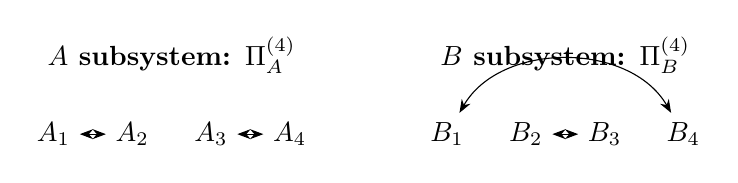
\begin{tikzpicture}[>=Stealth, node distance=1.5cm]
    % A subsystem
    \node (title_A) at (0, 2) {\textbf{$A$ subsystem: $\Pi_A^{(4)}$}};
    \node (A1) at (-1.5, 1) {$A_1$};
    \node (A2) at (-0.5, 1) {$A_2$};
    \node (A3) at (0.5, 1) {$A_3$};
    \node (A4) at (1.5, 1) {$A_4$};
    
    \draw[<->] (A1) -- (A2);
    \draw[<->] (A3) -- (A4);
    
    % B subsystem
    \node (title_B) at (5, 2) {\textbf{$B$ subsystem: $\Pi_B^{(4)}$}};
    \node (B1) at (3.5, 1) {$B_1$};
    \node (B2) at (4.5, 1) {$B_2$};
    \node (B3) at (5.5, 1) {$B_3$};
    \node (B4) at (6.5, 1) {$B_4$};
    
    \draw[<->] (B1) to[bend left=60] (B4);
    \draw[<->] (B2) -- (B3);
\end{tikzpicture}
\end{center}

In cycle notation:
\begin{align}
\Pi_A^{(4)} &\sim (1\ 2)(3\ 4) \\
\Pi_B^{(4)} &\sim (1\ 4)(2\ 3)
\end{align}

\section{Derivation of $S_6$}

\begin{theorem}[$S_6$ as a 6-Copy Observable]
\label{thm:S6}
For any bipartite density matrix $\rho$:
\begin{equation}
\boxed{S_6 = \Tr[(R^\dagger R)^3] = \Tr[\rho^{\otimes 6} \cdot (\Pi_A^{(6)} \otimes \Pi_B^{(6)})]}
\end{equation}
where:
\begin{align}
\Pi_A^{(6)} &= \SWAP_{A_1 A_2} \cdot \SWAP_{A_3 A_4} \cdot \SWAP_{A_5 A_6} \\
\Pi_B^{(6)} &= \SWAP_{B_1 B_6} \cdot \SWAP_{B_2 B_3} \cdot \SWAP_{B_4 B_5}
\end{align}
\end{theorem}

\begin{proof}
We expand $\Tr[(R^\dagger R)^3]$:
\begin{align}
\Tr[(R^\dagger R)^3] &= \sum (R^\dagger R)_{(j_1 l_1),(j_2 l_2)} (R^\dagger R)_{(j_2 l_2),(j_3 l_3)} (R^\dagger R)_{(j_3 l_3),(j_1 l_1)}
\end{align}

Each factor $(R^\dagger R)$ introduces two copies of $\rho$, giving 6 copies total.

Following the same analysis as for $S_4$:
\begin{itemize}
    \item The $A$-indices form three independent pairs, swapped by $\SWAP_{A_1 A_2} \cdot \SWAP_{A_3 A_4} \cdot \SWAP_{A_5 A_6}$
    \item The $B$-indices form a cyclic pattern requiring $\SWAP_{B_1 B_6} \cdot \SWAP_{B_2 B_3} \cdot \SWAP_{B_4 B_5}$
\end{itemize}
\end{proof}

\subsection{Permutation Pattern for $S_6$}

\begin{center}
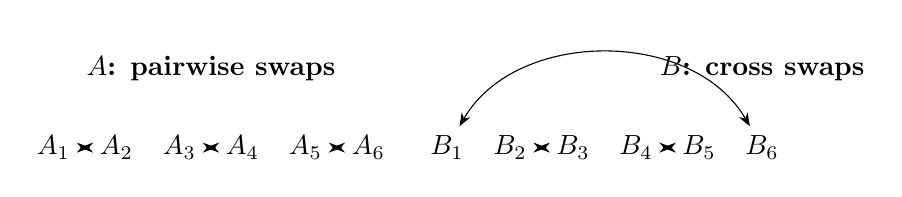
\begin{tikzpicture}[>=Stealth, node distance=1.2cm]
    % A subsystem
    \node (title_A) at (0, 2.5) {\textbf{$A$: pairwise swaps}};
    \foreach \i in {1,...,6} {
        \node (A\i) at ({(\i-3.5)*0.8}, 1.5) {$A_\i$};
    }
    \draw[<->] (A1) -- (A2);
    \draw[<->] (A3) -- (A4);
    \draw[<->] (A5) -- (A6);
    
    % B subsystem
    \node (title_B) at (7, 2.5) {\textbf{$B$: cross swaps}};
    \foreach \i in {1,...,6} {
        \node (B\i) at ({5 + (\i-3.5)*0.8}, 1.5) {$B_\i$};
    }
    \draw[<->] (B1) to[bend left=60] (B6);
    \draw[<->] (B2) -- (B3);
    \draw[<->] (B4) -- (B5);
\end{tikzpicture}
\end{center}

\section{General Formula for $S_{2k}$}

\begin{theorem}[General $S_{2k}$ Formula]
\label{thm:S2k}
For any positive integer $k$:
\begin{equation}
\boxed{S_{2k} = \Tr[(R^\dagger R)^k] = \Tr[\rho^{\otimes 2k} \cdot (\Pi_A^{(2k)} \otimes \Pi_B^{(2k)})]}
\end{equation}
where:
\begin{align}
\Pi_A^{(2k)} &= \prod_{m=0}^{k-1} \SWAP_{A_{2m+1}, A_{2m+2}} \\
\Pi_B^{(2k)} &= \SWAP_{B_1, B_{2k}} \cdot \prod_{m=1}^{k-1} \SWAP_{B_{2m}, B_{2m+1}}
\end{align}
\end{theorem}

\begin{proof}[Proof Sketch]
The structure follows from the pattern observed in $S_4$ and $S_6$:

\textbf{For $A$ subsystem:} Each factor of $(R^\dagger R)$ in the trace introduces a pair of copies that are swapped. With $k$ factors, we get $k$ independent pairwise swaps on copies $(1,2), (3,4), \ldots, (2k-1, 2k)$.

\textbf{For $B$ subsystem:} The trace structure creates a cyclic connection pattern. The copies connect as:
\begin{equation}
1 \leftrightarrow 2k, \quad 2 \leftrightarrow 3, \quad 4 \leftrightarrow 5, \quad \ldots
\end{equation}
\end{proof}

\subsection{Permutation Structure Summary}

\begin{table}[h]
\centering
\begin{tabular}{|c|c|c|}
\hline
$k$ & $\Pi_A^{(2k)}$ (cycle notation) & $\Pi_B^{(2k)}$ (cycle notation) \\
\hline
1 & $(1\ 2)$ & $(1\ 2)$ \\
2 & $(1\ 2)(3\ 4)$ & $(1\ 4)(2\ 3)$ \\
3 & $(1\ 2)(3\ 4)(5\ 6)$ & $(1\ 6)(2\ 3)(4\ 5)$ \\
$k$ & $\prod_{m=0}^{k-1}(2m{+}1\ \ 2m{+}2)$ & $(1\ 2k)\prod_{m=1}^{k-1}(2m\ \ 2m{+}1)$ \\
\hline
\end{tabular}
\caption{Permutation structure for $S_{2k}$}
\end{table}

\section{Comparison with Partial Transpose Moments}

\subsection{Partial Transpose Moment Formula}

The partial transpose moments $\mu_k = \Tr[(\rho^{T_A})^k]$ also have a multi-copy representation:
\begin{equation}
\mu_k = \Tr[\rho^{\otimes k} \cdot (\pi_k^{-1})_A \otimes (\pi_k)_B]
\end{equation}
where $\pi_k = (1\ 2\ 3\ \cdots\ k)$ is the cyclic permutation.

\subsection{Key Differences}

\begin{table}[h]
\centering
\begin{tabular}{|l|c|c|}
\hline
\textbf{Property} & \textbf{PT Moments $\mu_k$} & \textbf{Realignment Moments $S_{2k}$} \\
\hline
Copies needed for order $k$ & $k$ & $2k$ \\
$A$-permutation & $\pi_k^{-1}$ (inverse cyclic) & Pairwise SWAPs \\
$B$-permutation & $\pi_k$ (cyclic) & Cross SWAPs \\
Detects NPT entanglement & Yes & Yes \\
Detects bound entanglement & No (for PPT states) & Yes (some) \\
\hline
\end{tabular}
\caption{Comparison of partial transpose and realignment moments}
\end{table}

\section{Application: Moment-Based Entanglement Classifier}

\subsection{The Classifier}

Based on numerical optimization, we found that the ratio:
\begin{equation}
\mathcal{C} = \frac{S_2 \cdot S_6}{S_4^2}
\end{equation}
serves as an effective entanglement witness.

\begin{theorem}[Moment-Based Entanglement Criterion]
For $3 \times 3$ bipartite systems:
\begin{equation}
\boxed{\frac{S_2 \cdot S_6}{S_4^2} > 1.35 \implies \rho \text{ is entangled}}
\end{equation}
This criterion:
\begin{itemize}
    \item Has \textbf{zero false positives} on separable states
    \item Detects \textbf{100\%} of Tiles-type bound entangled states
    \item Detects $\approx$\textbf{69\%} of NPT entangled states
    \item Detects $\approx$\textbf{87\%} overall of realignment-detectable entanglement
\end{itemize}
\end{theorem}

\subsection{Observable Form of the Classifier}

The classifier can be expressed as:
\begin{equation}
\frac{\Tr[\rho^{\otimes 2} \cdot \SWAP] \cdot \Tr[\rho^{\otimes 6} \cdot (\Pi_A^{(6)} \otimes \Pi_B^{(6)})]}{\left(\Tr[\rho^{\otimes 4} \cdot (\Pi_A^{(4)} \otimes \Pi_B^{(4)})]\right)^2} > 1.35
\end{equation}

\subsection{Physical Interpretation}

The ratio $\frac{S_2 \cdot S_6}{S_4^2}$ measures the \textbf{shape} of the singular value distribution $\{\sigma_i\}$:

\begin{itemize}
    \item For a flat distribution ($\sigma_i = c$ for all $i$): $\frac{S_2 \cdot S_6}{S_4^2} = 1$
    \item For a peaked distribution (one dominant $\sigma$): ratio approaches 1
    \item For separable states: the constraint $\|R\|_1 \leq 1$ limits the ratio
    \item For entangled states: the ratio can exceed the separable bound
\end{itemize}

\section{Quantum Circuits for Measuring $S_k$}

The key insight for measuring $S_k$ is that the expectation value $\Tr[\rho^{\otimes n} \Pi]$ of any unitary permutation operator $\Pi$ can be measured using a \textbf{Hadamard test} with a single ancillary qubit.

\subsection{The Hadamard Test}

\begin{theorem}[Hadamard Test]
For a unitary operator $U$ and state $\rho$, the expectation value $\Tr[\rho U]$ can be measured as:
\begin{equation}
\Tr[\rho U] = 2P(0) - 1 + i(2P(+) - 1)
\end{equation}
where $P(0)$ and $P(+)$ are probabilities of measuring the ancilla in states $|0\rangle$ and $|+\rangle$ respectively.
\end{theorem}

For Hermitian permutation operators (like products of SWAPs), $\Tr[\rho^{\otimes n} \Pi]$ is real, so we only need to measure $P(0)$:
\begin{equation}
\boxed{\Tr[\rho^{\otimes n} \Pi] = 2P(0) - 1}
\end{equation}

\subsection{Circuit for $S_2$ (Purity / SWAP Test)}

The moment $S_2 = \Tr[\rho^2] = \Tr[\rho^{\otimes 2} \SWAP]$ is measured using the standard SWAP test.

For a bipartite state $\rho$ on $\mathcal{H}_A \otimes \mathcal{H}_B$, we need two copies. Label the wires as: $A_1, A_2$ for the two copies of subsystem $A$, and $B_1, B_2$ for subsystem $B$.

\begin{center}
\begin{quantikz}[row sep=0.5cm, column sep=0.5cm]
\lstick[wires=1]{Ancilla $\ket{0}$} & \gate{H} & \ctrl{1} & \ctrl{3} & \gate{H} & \meter{} \\
\lstick[wires=1]{$A_1$} & \qw & \swap{1} & \qw & \qw & \qw \\
\lstick[wires=1]{$A_2$} & \qw & \targX{} & \qw & \qw & \qw \\
\lstick[wires=1]{$B_1$} & \qw & \qw & \swap{1} & \qw & \qw \\
\lstick[wires=1]{$B_2$} & \qw & \qw & \targX{} & \qw & \qw
\end{quantikz}
\end{center}

The circuit implements:
\begin{itemize}
    \item Column 1: Controlled-SWAP between $A_1 \leftrightarrow A_2$
    \item Column 2: Controlled-SWAP between $B_1 \leftrightarrow B_2$
\end{itemize}

The measurement outcome gives:
\begin{equation}
S_2 = \Tr[\rho^2] = 2P(0) - 1
\end{equation}

\textbf{Simplified notation:} Using a bundled wire representation:

\begin{center}
\begin{quantikz}[row sep=0.6cm]
\lstick{$\ket{0}$} & \gate{H} & \ctrl{1} & \gate{H} & \meter{} \\
\lstick{$\rho^{\otimes 2}$} & \qw \qwbundle{2} & \gate{\text{c-SWAP}_A \otimes \text{c-SWAP}_B} & \qw & \qw
\end{quantikz}
\end{center}

\subsection{Circuit for $S_4$}

For $S_4 = \Tr[\rho^{\otimes 4} (\Pi_A^{(4)} \otimes \Pi_B^{(4)})]$, we need controlled versions of:
\begin{align}
\Pi_A^{(4)} &= \SWAP_{A_1 A_2} \cdot \SWAP_{A_3 A_4} \quad \text{(pairwise)} \\
\Pi_B^{(4)} &= \SWAP_{B_1 B_4} \cdot \SWAP_{B_2 B_3} \quad \text{(cross)}
\end{align}

The circuit has 9 wires: ancilla + 4 copies of $A$ + 4 copies of $B$:

\begin{center}
\begin{quantikz}[row sep=0.35cm, column sep=0.5cm]
\lstick{Anc.} & \gate{H} & \ctrl{1} & \ctrl{3} & \ctrl{6} & \ctrl{5} & \gate{H} & \meter{} \\
\lstick{$A_1$} & \qw & \swap{1} & \qw      & \qw      & \qw      & \qw & \qw \\
\lstick{$A_2$} & \qw & \targX{} & \qw      & \qw      & \qw      & \qw & \qw \\
\lstick{$A_3$} & \qw & \qw      & \swap{1} & \qw      & \qw      & \qw & \qw \\
\lstick{$A_4$} & \qw & \qw      & \targX{} & \qw      & \qw      & \qw & \qw \\
\lstick{$B_1$} & \qw & \qw      & \qw      & \qw      & \swap{3} & \qw & \qw \\
\lstick{$B_2$} & \qw & \qw      & \qw      & \swap{1} & \qw      & \qw & \qw \\
\lstick{$B_3$} & \qw & \qw      & \qw      & \targX{} & \qw      & \qw & \qw \\
\lstick{$B_4$} & \qw & \qw      & \qw      & \qw      & \targX{} & \qw & \qw
\end{quantikz}
\end{center}

\textbf{Circuit structure:}
\begin{itemize}
    \item Column 1: c-SWAP$(A_1 \leftrightarrow A_2)$ --- control at ancilla (wire 0), targets at wires 1,2
    \item Column 2: c-SWAP$(A_3 \leftrightarrow A_4)$ --- control at ancilla, targets at wires 3,4
    \item Column 3: c-SWAP$(B_2 \leftrightarrow B_3)$ --- control at ancilla, targets at wires 6,7
    \item Column 4: c-SWAP$(B_1 \leftrightarrow B_4)$ --- control at ancilla, targets at wires 5,8
\end{itemize}

The measurement yields:
\begin{equation}
S_4 = 2P(0) - 1
\end{equation}

\subsection{Circuit for $S_6$}

For $S_6 = \Tr[\rho^{\otimes 6} (\Pi_A^{(6)} \otimes \Pi_B^{(6)})]$:
\begin{align}
\Pi_A^{(6)} &= \SWAP_{A_1 A_2} \cdot \SWAP_{A_3 A_4} \cdot \SWAP_{A_5 A_6} \quad \text{(pairwise)} \\
\Pi_B^{(6)} &= \SWAP_{B_1 B_6} \cdot \SWAP_{B_2 B_3} \cdot \SWAP_{B_4 B_5} \quad \text{(cross)}
\end{align}

The circuit has 13 wires: ancilla + 6 copies of $A$ + 6 copies of $B$:

\begin{center}
\begin{quantikz}[row sep=0.28cm, column sep=0.4cm]
\lstick{Anc.} & \gate{H} & \ctrl{1} & \ctrl{3} & \ctrl{5} & \ctrl{8} & \ctrl{10} & \ctrl{7} & \gate{H} & \meter{} \\
\lstick{$A_1$} & \qw & \swap{1} & \qw      & \qw      & \qw      & \qw       & \qw      & \qw & \qw \\
\lstick{$A_2$} & \qw & \targX{} & \qw      & \qw      & \qw      & \qw       & \qw      & \qw & \qw \\
\lstick{$A_3$} & \qw & \qw      & \swap{1} & \qw      & \qw      & \qw       & \qw      & \qw & \qw \\
\lstick{$A_4$} & \qw & \qw      & \targX{} & \qw      & \qw      & \qw       & \qw      & \qw & \qw \\
\lstick{$A_5$} & \qw & \qw      & \qw      & \swap{1} & \qw      & \qw       & \qw      & \qw & \qw \\
\lstick{$A_6$} & \qw & \qw      & \qw      & \targX{} & \qw      & \qw       & \qw      & \qw & \qw \\
\lstick{$B_1$} & \qw & \qw      & \qw      & \qw      & \qw      & \qw       & \swap{5} & \qw & \qw \\
\lstick{$B_2$} & \qw & \qw      & \qw      & \qw      & \swap{1} & \qw       & \qw      & \qw & \qw \\
\lstick{$B_3$} & \qw & \qw      & \qw      & \qw      & \targX{} & \qw       & \qw      & \qw & \qw \\
\lstick{$B_4$} & \qw & \qw      & \qw      & \qw      & \qw      & \swap{1}  & \qw      & \qw & \qw \\
\lstick{$B_5$} & \qw & \qw      & \qw      & \qw      & \qw      & \targX{}  & \qw      & \qw & \qw \\
\lstick{$B_6$} & \qw & \qw      & \qw      & \qw      & \qw      & \qw       & \targX{} & \qw & \qw
\end{quantikz}
\end{center}

\textbf{Circuit structure:}
\begin{itemize}
    \item Columns 1--3: c-SWAP$(A_1{\leftrightarrow}A_2)$, c-SWAP$(A_3{\leftrightarrow}A_4)$, c-SWAP$(A_5{\leftrightarrow}A_6)$
    \item Columns 4--6: c-SWAP$(B_2{\leftrightarrow}B_3)$, c-SWAP$(B_4{\leftrightarrow}B_5)$, c-SWAP$(B_1{\leftrightarrow}B_6)$
\end{itemize}

\subsection{General Circuit Structure for $S_{2k}$}

The general circuit for measuring $S_{2k}$ has the structure:

\begin{center}
\begin{quantikz}[row sep=0.5cm]
\lstick{$\ket{0}$} & \gate{H} & \ctrl{1} & \gate{H} & \meter{} \\
\lstick{$\rho^{\otimes 2k}$} & \qw \qwbundle{2k} & \gate{\Pi_A^{(2k)} \otimes \Pi_B^{(2k)}} & \qw & \qw
\end{quantikz}
\end{center}

where:
\begin{equation}
\Pi_A^{(2k)} \otimes \Pi_B^{(2k)} = \left(\prod_{m=0}^{k-1} \SWAP_{A_{2m+1}, A_{2m+2}}\right) \otimes \left(\SWAP_{B_1, B_{2k}} \cdot \prod_{m=1}^{k-1} \SWAP_{B_{2m}, B_{2m+1}}\right)
\end{equation}

\subsection{Circuit for the Entanglement Classifier}

To evaluate the classifier $\mathcal{C} = \frac{S_2 \cdot S_6}{S_4^2} > 1.35$, we need three separate circuits:

\begin{enumerate}
    \item \textbf{Measure $S_2$}: Use 2 copies, 1 c-SWAP per subsystem
    \item \textbf{Measure $S_4$}: Use 4 copies, 2 c-SWAPs per subsystem  
    \item \textbf{Measure $S_6$}: Use 6 copies, 3 c-SWAPs per subsystem
\end{enumerate}

\begin{center}
\begin{tabular}{|c|c|c|c|}
\hline
Moment & Copies & c-SWAPs (total) & CNOTs (total) \\
\hline
$S_2$ & 2 & 2 & 6 \\
$S_4$ & 4 & 4 & 12 \\
$S_6$ & 6 & 6 & 18 \\
\hline
\textbf{Total} & \textbf{12} & \textbf{12} & \textbf{36} \\
\hline
\end{tabular}
\end{center}

\textbf{Note:} Each controlled-SWAP (Fredkin gate) decomposes into at most 5 two-qubit gates, or approximately 3 CNOTs when optimized.

\subsection{Alternative: Destructive SWAP Test}

For improved sample efficiency, one can use the \textbf{destructive SWAP test} which measures all qubits but doesn't require an ancilla:

\begin{center}
\begin{quantikz}[row sep=0.4cm]
\lstick{$\rho$} & \ctrl{1} & \gate{H} & \meter{} \\
\lstick{$\rho$} & \targ{} & \qw & \meter{}
\end{quantikz}
\end{center}

For this circuit, $\Tr[\rho^2] = 2P(\text{same outcome}) - 1$.

The destructive version can be extended to measure $S_4$ and $S_6$ by:
\begin{enumerate}
    \item Applying the appropriate CNOT pattern (not controlled)
    \item Applying Hadamards to half the qubits
    \item Measuring all qubits
    \item Post-processing to extract $S_k$
\end{enumerate}

\subsection{Complete Circuits for $3 \times 3$ Systems with 2-Qubit Qutrit Encoding}

For experimental implementation on qubit-based quantum computers, we encode each qutrit in 2 qubits.

\subsubsection{Encoding Scheme}

Each qutrit ($d=3$) is encoded in 2 physical qubits:
\begin{equation}
|0\rangle_{\text{qutrit}} \to |00\rangle, \quad
|1\rangle_{\text{qutrit}} \to |01\rangle, \quad
|2\rangle_{\text{qutrit}} \to |10\rangle
\end{equation}
The state $|11\rangle$ lies outside the computational subspace.

For a $3 \times 3$ bipartite state $\rho$ on $\C^3 \otimes \C^3$:
\begin{itemize}
    \item Subsystem $A$ (qutrit): encoded in 2 qubits $(a^0, a^1)$
    \item Subsystem $B$ (qutrit): encoded in 2 qubits $(b^0, b^1)$
    \item \textbf{Total: 4 physical qubits per copy of $\rho$}
\end{itemize}

\textbf{Key principle:} To swap two encoded qutrits, we must swap \emph{both} encoding qubits:
\begin{equation}
\text{SWAP}_{\text{qutrit}}(i,j) = \text{SWAP}(a_i^0, a_j^0) \otimes \text{SWAP}(a_i^1, a_j^1)
\end{equation}

\subsubsection{Wire Labeling Convention}

For $n$ copies of $\rho$, we use the following wire ordering:
\begin{center}
\begin{tabular}{|c|l|}
\hline
Wire & Description \\
\hline
0 & Ancilla \\
$4(i-1)+1$ & $a_i^0$ (qutrit $A_i$, MSB) \\
$4(i-1)+2$ & $a_i^1$ (qutrit $A_i$, LSB) \\
$4(i-1)+3$ & $b_i^0$ (qutrit $B_i$, MSB) \\
$4(i-1)+4$ & $b_i^1$ (qutrit $B_i$, LSB) \\
\hline
\end{tabular}
\end{center}

\subsubsection{Circuit for $S_2$ (9 qubits)}

\textbf{Resources:} 2 copies $\times$ 4 qubits + 1 ancilla = \textbf{9 qubits}

\textbf{Wire assignment:}
\begin{center}
\begin{tabular}{|c|c|l|}
\hline
Wire & Label & Description \\
\hline
0 & Anc & Ancilla \\
1 & $a_1^0$ & Copy 1, qutrit A, MSB \\
2 & $a_1^1$ & Copy 1, qutrit A, LSB \\
3 & $b_1^0$ & Copy 1, qutrit B, MSB \\
4 & $b_1^1$ & Copy 1, qutrit B, LSB \\
5 & $a_2^0$ & Copy 2, qutrit A, MSB \\
6 & $a_2^1$ & Copy 2, qutrit A, LSB \\
7 & $b_2^0$ & Copy 2, qutrit B, MSB \\
8 & $b_2^1$ & Copy 2, qutrit B, LSB \\
\hline
\end{tabular}
\end{center}

\textbf{Operations:}
\begin{itemize}
    \item $\text{SWAP}_{A_1 \leftrightarrow A_2}$: c-SWAP$(1,5)$, c-SWAP$(2,6)$
    \item $\text{SWAP}_{B_1 \leftrightarrow B_2}$: c-SWAP$(3,7)$, c-SWAP$(4,8)$
\end{itemize}

\begin{center}
\begin{quantikz}[row sep=0.4cm, column sep=0.5cm]
\lstick{\small 0}  & \gate{H} & \ctrl{1} & \ctrl{2} & \ctrl{3} & \ctrl{4} & \gate{H} & \meter{} \\
\lstick{\small 1}  & \qw & \swap{4} & \qw      & \qw      & \qw      & \qw & \qw \\
\lstick{\small 2}  & \qw & \qw      & \swap{4} & \qw      & \qw      & \qw & \qw \\
\lstick{\small 3}  & \qw & \qw      & \qw      & \swap{4} & \qw      & \qw & \qw \\
\lstick{\small 4}  & \qw & \qw      & \qw      & \qw      & \swap{4} & \qw & \qw \\
\lstick{\small 5}  & \qw & \targX{} & \qw      & \qw      & \qw      & \qw & \qw \\
\lstick{\small 6}  & \qw & \qw      & \targX{} & \qw      & \qw      & \qw & \qw \\
\lstick{\small 7}  & \qw & \qw      & \qw      & \targX{} & \qw      & \qw & \qw \\
\lstick{\small 8}  & \qw & \qw      & \qw      & \qw      & \targX{} & \qw & \qw
\end{quantikz}
\end{center}

\textbf{Wire labels:} 0=Anc, 1-4=$(a_1^0,a_1^1,b_1^0,b_1^1)$, 5-8=$(a_2^0,a_2^1,b_2^0,b_2^1)$.

\textbf{Gate count:} 4 controlled-SWAP gates $\approx$ 32 CNOTs

\subsubsection{Circuit for $S_4$ (17 qubits)}

\textbf{Resources:} 4 copies $\times$ 4 qubits + 1 ancilla = \textbf{17 qubits}

\textbf{Permutations:}
\begin{align}
\Pi_A^{(4)} &= \text{SWAP}_{A_1,A_2} \cdot \text{SWAP}_{A_3,A_4} \\
\Pi_B^{(4)} &= \text{SWAP}_{B_1,B_4} \cdot \text{SWAP}_{B_2,B_3}
\end{align}

\textbf{Wire assignment:}
\begin{center}
\begin{tabular}{|c|c||c|c||c|c||c|c|}
\hline
\multicolumn{2}{|c||}{Copy 1} & \multicolumn{2}{c||}{Copy 2} & \multicolumn{2}{c||}{Copy 3} & \multicolumn{2}{c|}{Copy 4} \\
\hline
1 & $a_1^0$ & 5 & $a_2^0$ & 9 & $a_3^0$ & 13 & $a_4^0$ \\
2 & $a_1^1$ & 6 & $a_2^1$ & 10 & $a_3^1$ & 14 & $a_4^1$ \\
3 & $b_1^0$ & 7 & $b_2^0$ & 11 & $b_3^0$ & 15 & $b_4^0$ \\
4 & $b_1^1$ & 8 & $b_2^1$ & 12 & $b_3^1$ & 16 & $b_4^1$ \\
\hline
\end{tabular}
\end{center}

\textbf{Operations (8 c-SWAPs):}
\begin{itemize}
    \item $A_1 \leftrightarrow A_2$: c-SWAP$(1,5)$, c-SWAP$(2,6)$
    \item $A_3 \leftrightarrow A_4$: c-SWAP$(9,13)$, c-SWAP$(10,14)$
    \item $B_1 \leftrightarrow B_4$: c-SWAP$(3,15)$, c-SWAP$(4,16)$
    \item $B_2 \leftrightarrow B_3$: c-SWAP$(7,11)$, c-SWAP$(8,12)$
\end{itemize}

\begin{center}
\begin{quantikz}[row sep=0.28cm, column sep=0.3cm]
\lstick{\small 0}  & \gate{H} & \ctrl{1} & \ctrl{2} & \ctrl{9}  & \ctrl{10} & \ctrl{3}  & \ctrl{4}  & \ctrl{7}  & \ctrl{8}  & \gate{H} & \meter{} \\
\lstick{\small 1}  & \qw & \swap{4} & \qw      & \qw       & \qw       & \qw       & \qw       & \qw       & \qw       & \qw & \qw \\
\lstick{\small 2}  & \qw & \qw      & \swap{4} & \qw       & \qw       & \qw       & \qw       & \qw       & \qw       & \qw & \qw \\
\lstick{\small 3}  & \qw & \qw      & \qw      & \qw       & \qw       & \swap{12} & \qw       & \qw       & \qw       & \qw & \qw \\
\lstick{\small 4}  & \qw & \qw      & \qw      & \qw       & \qw       & \qw       & \swap{12} & \qw       & \qw       & \qw & \qw \\
\lstick{\small 5}  & \qw & \targX{} & \qw      & \qw       & \qw       & \qw       & \qw       & \qw       & \qw       & \qw & \qw \\
\lstick{\small 6}  & \qw & \qw      & \targX{} & \qw       & \qw       & \qw       & \qw       & \qw       & \qw       & \qw & \qw \\
\lstick{\small 7}  & \qw & \qw      & \qw      & \qw       & \qw       & \qw       & \qw       & \swap{4}  & \qw       & \qw & \qw \\
\lstick{\small 8}  & \qw & \qw      & \qw      & \qw       & \qw       & \qw       & \qw       & \qw       & \swap{4}  & \qw & \qw \\
\lstick{\small 9}  & \qw & \qw      & \qw      & \swap{4}  & \qw       & \qw       & \qw       & \qw       & \qw       & \qw & \qw \\
\lstick{\small 10} & \qw & \qw      & \qw      & \qw       & \swap{4}  & \qw       & \qw       & \qw       & \qw       & \qw & \qw \\
\lstick{\small 11} & \qw & \qw      & \qw      & \qw       & \qw       & \qw       & \qw       & \targX{}  & \qw       & \qw & \qw \\
\lstick{\small 12} & \qw & \qw      & \qw      & \qw       & \qw       & \qw       & \qw       & \qw       & \targX{}  & \qw & \qw \\
\lstick{\small 13} & \qw & \qw      & \qw      & \targX{}  & \qw       & \qw       & \qw       & \qw       & \qw       & \qw & \qw \\
\lstick{\small 14} & \qw & \qw      & \qw      & \qw       & \targX{}  & \qw       & \qw       & \qw       & \qw       & \qw & \qw \\
\lstick{\small 15} & \qw & \qw      & \qw      & \qw       & \qw       & \targX{}  & \qw       & \qw       & \qw       & \qw & \qw \\
\lstick{\small 16} & \qw & \qw      & \qw      & \qw       & \qw       & \qw       & \targX{}  & \qw       & \qw       & \qw & \qw
\end{quantikz}
\end{center}

\textbf{Wire labels:} 0=Anc, 1-4=$(a_1^0,a_1^1,b_1^0,b_1^1)$, 5-8=$(a_2^0,a_2^1,b_2^0,b_2^1)$, 9-12=$(a_3^0,a_3^1,b_3^0,b_3^1)$, 13-16=$(a_4^0,a_4^1,b_4^0,b_4^1)$.

\textbf{Gate count:} 8 controlled-SWAP gates $\approx$ 64 CNOTs

\subsubsection{Circuit for $S_6$ (25 qubits)}

\textbf{Resources:} 6 copies $\times$ 4 qubits + 1 ancilla = \textbf{25 qubits}

\textbf{Permutations:}
\begin{align}
\Pi_A^{(6)} &= \text{SWAP}_{A_1,A_2} \cdot \text{SWAP}_{A_3,A_4} \cdot \text{SWAP}_{A_5,A_6} \\
\Pi_B^{(6)} &= \text{SWAP}_{B_1,B_6} \cdot \text{SWAP}_{B_2,B_3} \cdot \text{SWAP}_{B_4,B_5}
\end{align}

\textbf{Wire assignment (Copy $i$: wires $4(i-1)+1$ to $4(i-1)+4$):}
\begin{center}
\begin{tabular}{|c|cccc|cccc|cccc|}
\hline
Copy & \multicolumn{4}{c|}{1} & \multicolumn{4}{c|}{2} & \multicolumn{4}{c|}{3} \\
\hline
Wire & 1 & 2 & 3 & 4 & 5 & 6 & 7 & 8 & 9 & 10 & 11 & 12 \\
Label & $a_1^0$ & $a_1^1$ & $b_1^0$ & $b_1^1$ & $a_2^0$ & $a_2^1$ & $b_2^0$ & $b_2^1$ & $a_3^0$ & $a_3^1$ & $b_3^0$ & $b_3^1$ \\
\hline
\hline
Copy & \multicolumn{4}{c|}{4} & \multicolumn{4}{c|}{5} & \multicolumn{4}{c|}{6} \\
\hline
Wire & 13 & 14 & 15 & 16 & 17 & 18 & 19 & 20 & 21 & 22 & 23 & 24 \\
Label & $a_4^0$ & $a_4^1$ & $b_4^0$ & $b_4^1$ & $a_5^0$ & $a_5^1$ & $b_5^0$ & $b_5^1$ & $a_6^0$ & $a_6^1$ & $b_6^0$ & $b_6^1$ \\
\hline
\end{tabular}
\end{center}

\textbf{Operations (12 c-SWAPs):}

$\Pi_A^{(6)}$:
\begin{itemize}
    \item $A_1 \leftrightarrow A_2$: c-SWAP$(1,5)$, c-SWAP$(2,6)$
    \item $A_3 \leftrightarrow A_4$: c-SWAP$(9,13)$, c-SWAP$(10,14)$
    \item $A_5 \leftrightarrow A_6$: c-SWAP$(17,21)$, c-SWAP$(18,22)$
\end{itemize}

$\Pi_B^{(6)}$:
\begin{itemize}
    \item $B_1 \leftrightarrow B_6$: c-SWAP$(3,23)$, c-SWAP$(4,24)$
    \item $B_2 \leftrightarrow B_3$: c-SWAP$(7,11)$, c-SWAP$(8,12)$
    \item $B_4 \leftrightarrow B_5$: c-SWAP$(15,19)$, c-SWAP$(16,20)$
\end{itemize}

\begin{center}
\begin{quantikz}[row sep=0.22cm, column sep=0.22cm]
\lstick{\tiny 0} & \gate{H} & \ctrl{1} & \ctrl{2} & \ctrl{9} & \ctrl{10} & \ctrl{17} & \ctrl{18} & \ctrl{3} & \ctrl{4} & \ctrl{7} & \ctrl{8} & \ctrl{15} & \ctrl{16} & \gate{H} & \meter{} \\
\lstick{\tiny 1} & \qw & \swap{4}  & \qw       & \qw       & \qw        & \qw        & \qw        & \qw        & \qw        & \qw       & \qw       & \qw        & \qw        & \qw & \qw \\
\lstick{\tiny 2} & \qw & \qw       & \swap{4}  & \qw       & \qw        & \qw        & \qw        & \qw        & \qw        & \qw       & \qw       & \qw        & \qw        & \qw & \qw \\
\lstick{\tiny 3} & \qw & \qw       & \qw       & \qw       & \qw        & \qw        & \qw        & \swap{20}  & \qw        & \qw       & \qw       & \qw        & \qw        & \qw & \qw \\
\lstick{\tiny 4} & \qw & \qw       & \qw       & \qw       & \qw        & \qw        & \qw        & \qw        & \swap{20}  & \qw       & \qw       & \qw        & \qw        & \qw & \qw \\
\lstick{\tiny 5} & \qw & \targX{}  & \qw       & \qw       & \qw        & \qw        & \qw        & \qw        & \qw        & \qw       & \qw       & \qw        & \qw        & \qw & \qw \\
\lstick{\tiny 6} & \qw & \qw       & \targX{}  & \qw       & \qw        & \qw        & \qw        & \qw        & \qw        & \qw       & \qw       & \qw        & \qw        & \qw & \qw \\
\lstick{\tiny 7} & \qw & \qw       & \qw       & \qw       & \qw        & \qw        & \qw        & \qw        & \qw        & \swap{4}  & \qw       & \qw        & \qw        & \qw & \qw \\
\lstick{\tiny 8} & \qw & \qw       & \qw       & \qw       & \qw        & \qw        & \qw        & \qw        & \qw        & \qw       & \swap{4}  & \qw        & \qw        & \qw & \qw \\
\lstick{\tiny 9} & \qw & \qw       & \qw       & \swap{4}  & \qw        & \qw        & \qw        & \qw        & \qw        & \qw       & \qw       & \qw        & \qw        & \qw & \qw \\
\lstick{\tiny 10} & \qw & \qw       & \qw       & \qw       & \swap{4}   & \qw        & \qw        & \qw        & \qw        & \qw       & \qw       & \qw        & \qw        & \qw & \qw \\
\lstick{\tiny 11} & \qw & \qw       & \qw       & \qw       & \qw        & \qw        & \qw        & \qw        & \qw        & \targX{}  & \qw       & \qw        & \qw        & \qw & \qw \\
\lstick{\tiny 12} & \qw & \qw       & \qw       & \qw       & \qw        & \qw        & \qw        & \qw        & \qw        & \qw       & \targX{}  & \qw        & \qw        & \qw & \qw \\
\lstick{\tiny 13} & \qw & \qw       & \qw       & \targX{}  & \qw        & \qw        & \qw        & \qw        & \qw        & \qw       & \qw       & \qw        & \qw        & \qw & \qw \\
\lstick{\tiny 14} & \qw & \qw       & \qw       & \qw       & \targX{}   & \qw        & \qw        & \qw        & \qw        & \qw       & \qw       & \qw        & \qw        & \qw & \qw \\
\lstick{\tiny 15} & \qw & \qw       & \qw       & \qw       & \qw        & \qw        & \qw        & \qw        & \qw        & \qw       & \qw       & \swap{4}   & \qw        & \qw & \qw \\
\lstick{\tiny 16} & \qw & \qw       & \qw       & \qw       & \qw        & \qw        & \qw        & \qw        & \qw        & \qw       & \qw       & \qw        & \swap{4}   & \qw & \qw \\
\lstick{\tiny 17} & \qw & \qw       & \qw       & \qw       & \qw        & \swap{4}   & \qw        & \qw        & \qw        & \qw       & \qw       & \qw        & \qw        & \qw & \qw \\
\lstick{\tiny 18} & \qw & \qw       & \qw       & \qw       & \qw        & \qw        & \swap{4}   & \qw        & \qw        & \qw       & \qw       & \qw        & \qw        & \qw & \qw \\
\lstick{\tiny 19} & \qw & \qw       & \qw       & \qw       & \qw        & \qw        & \qw        & \qw        & \qw        & \qw       & \qw       & \targX{}   & \qw        & \qw & \qw \\
\lstick{\tiny 20} & \qw & \qw       & \qw       & \qw       & \qw        & \qw        & \qw        & \qw        & \qw        & \qw       & \qw       & \qw        & \targX{}   & \qw & \qw \\
\lstick{\tiny 21} & \qw & \qw       & \qw       & \qw       & \qw        & \targX{}   & \qw        & \qw        & \qw        & \qw       & \qw       & \qw        & \qw        & \qw & \qw \\
\lstick{\tiny 22} & \qw & \qw       & \qw       & \qw       & \qw        & \qw        & \targX{}   & \qw        & \qw        & \qw       & \qw       & \qw        & \qw        & \qw & \qw \\
\lstick{\tiny 23} & \qw & \qw       & \qw       & \qw       & \qw        & \qw        & \qw        & \targX{}   & \qw        & \qw       & \qw       & \qw        & \qw        & \qw & \qw \\
\lstick{\tiny 24} & \qw & \qw       & \qw       & \qw       & \qw        & \qw        & \qw        & \qw        & \targX{}   & \qw       & \qw       & \qw        & \qw        & \qw & \qw
\end{quantikz}
\end{center}

\textbf{Wire labels:} 0=Anc, 1-4=$(a_1^0,a_1^1,b_1^0,b_1^1)$, 5-8=$(a_2^0,a_2^1,b_2^0,b_2^1)$, 9-12=$(a_3^0,a_3^1,b_3^0,b_3^1)$, 13-16=$(a_4^0,a_4^1,b_4^0,b_4^1)$, 17-20=$(a_5^0,a_5^1,b_5^0,b_5^1)$, 21-24=$(a_6^0,a_6^1,b_6^0,b_6^1)$.

\textbf{Gate count:} 12 controlled-SWAP gates $\approx$ 96 CNOTs

\subsubsection{Circuit for $T_4$ (PT Moment, 17 qubits)}

For $T_4 = \Tr[(\rho^{T_A})^4]$, we need \textbf{cyclic} permutations instead of pairwise SWAPs:
\begin{align}
(\pi_4^{-1})_A &: A_1 \to A_4 \to A_3 \to A_2 \to A_1 \quad \text{(inverse 4-cycle)} \\
(\pi_4)_B &: B_1 \to B_2 \to B_3 \to B_4 \to B_1 \quad \text{(4-cycle)}
\end{align}

\textbf{Cyclic decomposition:} A 4-cycle decomposes into 3 transpositions:
\begin{align}
(1\ 2\ 3\ 4) &= (3\ 4)(2\ 3)(1\ 2) \quad \text{(apply right to left)} \\
(4\ 3\ 2\ 1) &= (1\ 2)(2\ 3)(3\ 4) \quad \text{(inverse)}
\end{align}

\textbf{Operations for $T_4$ (12 c-SWAPs):}

$(\pi_4^{-1})_A$ (inverse cycle on A):
\begin{itemize}
    \item c-SWAP$(A_3,A_4)$: wires $(9,13)$, $(10,14)$
    \item c-SWAP$(A_2,A_3)$: wires $(5,9)$, $(6,10)$
    \item c-SWAP$(A_1,A_2)$: wires $(1,5)$, $(2,6)$
\end{itemize}

$(\pi_4)_B$ (forward cycle on B):
\begin{itemize}
    \item c-SWAP$(B_1,B_2)$: wires $(3,7)$, $(4,8)$
    \item c-SWAP$(B_2,B_3)$: wires $(7,11)$, $(8,12)$
    \item c-SWAP$(B_3,B_4)$: wires $(11,15)$, $(12,16)$
\end{itemize}

\begin{center}
\begin{quantikz}[row sep=0.28cm, column sep=0.22cm]
\lstick{\small 0}  & \gate{H} & \ctrl{9} & \ctrl{10} & \ctrl{5} & \ctrl{6} & \ctrl{1} & \ctrl{2} & \ctrl{3} & \ctrl{4} & \ctrl{7} & \ctrl{8} & \ctrl{11} & \ctrl{12} & \gate{H} & \meter{} \\
\lstick{\small 1}  & \qw & \qw      & \qw       & \qw      & \qw      & \swap{4} & \qw      & \qw      & \qw      & \qw      & \qw      & \qw       & \qw       & \qw & \qw \\
\lstick{\small 2}  & \qw & \qw      & \qw       & \qw      & \qw      & \qw      & \swap{4} & \qw      & \qw      & \qw      & \qw      & \qw       & \qw       & \qw & \qw \\
\lstick{\small 3}  & \qw & \qw      & \qw       & \qw      & \qw      & \qw      & \qw      & \swap{4} & \qw      & \qw      & \qw      & \qw       & \qw       & \qw & \qw \\
\lstick{\small 4}  & \qw & \qw      & \qw       & \qw      & \qw      & \qw      & \qw      & \qw      & \swap{4} & \qw      & \qw      & \qw       & \qw       & \qw & \qw \\
\lstick{\small 5}  & \qw & \qw      & \qw       & \swap{4} & \qw      & \targX{} & \qw      & \qw      & \qw      & \qw      & \qw      & \qw       & \qw       & \qw & \qw \\
\lstick{\small 6}  & \qw & \qw      & \qw       & \qw      & \swap{4} & \qw      & \targX{} & \qw      & \qw      & \qw      & \qw      & \qw       & \qw       & \qw & \qw \\
\lstick{\small 7}  & \qw & \qw      & \qw       & \qw      & \qw      & \qw      & \qw      & \targX{} & \qw      & \swap{4} & \qw      & \qw       & \qw       & \qw & \qw \\
\lstick{\small 8}  & \qw & \qw      & \qw       & \qw      & \qw      & \qw      & \qw      & \qw      & \targX{} & \qw      & \swap{4} & \qw       & \qw       & \qw & \qw \\
\lstick{\small 9}  & \qw & \swap{4} & \qw       & \targX{} & \qw      & \qw      & \qw      & \qw      & \qw      & \qw      & \qw      & \qw       & \qw       & \qw & \qw \\
\lstick{\small 10} & \qw & \qw      & \swap{4}  & \qw      & \targX{} & \qw      & \qw      & \qw      & \qw      & \qw      & \qw      & \qw       & \qw       & \qw & \qw \\
\lstick{\small 11} & \qw & \qw      & \qw       & \qw      & \qw      & \qw      & \qw      & \qw      & \qw      & \targX{} & \qw      & \swap{4}  & \qw       & \qw & \qw \\
\lstick{\small 12} & \qw & \qw      & \qw       & \qw      & \qw      & \qw      & \qw      & \qw      & \qw      & \qw      & \targX{} & \qw       & \swap{4}  & \qw & \qw \\
\lstick{\small 13} & \qw & \targX{} & \qw       & \qw      & \qw      & \qw      & \qw      & \qw      & \qw      & \qw      & \qw      & \qw       & \qw       & \qw & \qw \\
\lstick{\small 14} & \qw & \qw      & \targX{}  & \qw      & \qw      & \qw      & \qw      & \qw      & \qw      & \qw      & \qw      & \qw       & \qw       & \qw & \qw \\
\lstick{\small 15} & \qw & \qw      & \qw       & \qw      & \qw      & \qw      & \qw      & \qw      & \qw      & \qw      & \qw      & \targX{}  & \qw       & \qw & \qw \\
\lstick{\small 16} & \qw & \qw      & \qw       & \qw      & \qw      & \qw      & \qw      & \qw      & \qw      & \qw      & \qw      & \qw       & \targX{}  & \qw & \qw
\end{quantikz}
\end{center}

\textbf{Wire labels:} 0=Anc, 1-4=$(a_1^0,a_1^1,b_1^0,b_1^1)$, 5-8=$(a_2^0,a_2^1,b_2^0,b_2^1)$, 9-12=$(a_3^0,a_3^1,b_3^0,b_3^1)$, 13-16=$(a_4^0,a_4^1,b_4^0,b_4^1)$.

\textbf{Gate count:} 12 controlled-SWAP gates $\approx$ 96 CNOTs

\subsubsection{Resource Summary for $3 \times 3$ Systems}

\begin{center}
\begin{tabular}{|c|c|c|c|c|}
\hline
\textbf{Moment} & \textbf{Copies} & \textbf{Qubits} & \textbf{c-SWAPs} & \textbf{CNOTs} \\
\hline
$S_2$ & 2 & 9 & 4 & $\sim$32 \\
$S_4$ & 4 & 17 & 8 & $\sim$64 \\
$S_6$ & 6 & 25 & 12 & $\sim$96 \\
\hline
$T_2$ & 2 & 9 & 4 & $\sim$32 \\
$T_4$ & 4 & 17 & 12 & $\sim$96 \\
$T_6$ & 6 & 25 & 18 & $\sim$144 \\
\hline
\end{tabular}
\end{center}

\textbf{Note:} Each c-SWAP (Fredkin gate) decomposes into $\sim$8 CNOTs. The cyclic permutations for $T_k$ require more gates than the pairwise SWAPs for $S_k$.

For the entanglement classifier $\mathcal{C} = S_2 \cdot S_6 / S_4^2$:
\begin{itemize}
    \item Total qubits needed: $\max(9, 17, 25) = 25$
    \item Total measurements: 3 separate circuits
    \item Total c-SWAPs: $4 + 8 + 12 = 24$
\end{itemize}

\subsection{Heavy-Hex Topology Mapping}

IBM quantum processors use the \textbf{heavy-hex} topology, which constrains qubit connectivity. We describe optimal mappings of the qutrit-encoded circuits onto this architecture.

\subsubsection{Heavy-Hex Topology Structure}

The heavy-hex lattice consists of:
\begin{itemize}
    \item \textbf{Degree-3 qubits}: At hexagon vertices (chain qubits)
    \item \textbf{Degree-2 qubits}: Bridge qubits connecting chains
\end{itemize}

\begin{center}
\textbf{IBM Heavy-Hex Topology} (partial view of 127-qubit device)
\vspace{0.3cm}

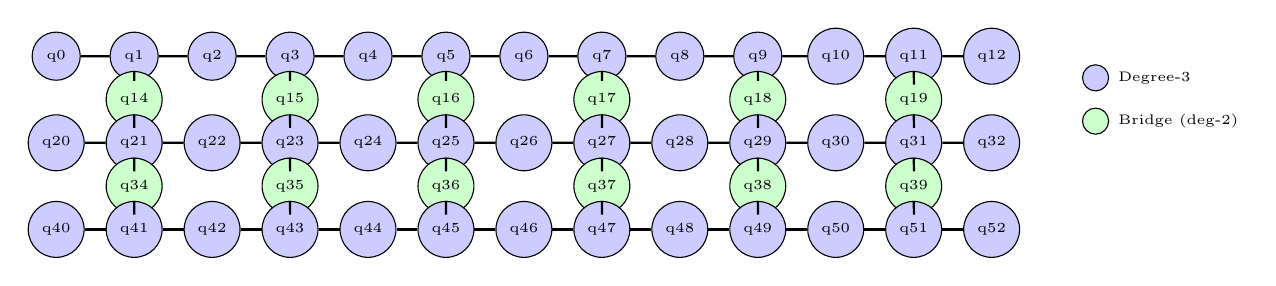
\begin{tikzpicture}[scale=0.55, every node/.style={font=\tiny}]
    % Row 0 qubits (degree-3)
    \foreach \i in {0,...,12} {
        \node[circle, draw, fill=blue!20, minimum size=4mm] (r0q\i) at (\i*1.8, 4) {q\i};
    }
    % Horizontal edges Row 0
    \foreach \i in {0,...,11} {
        \pgfmathtruncatemacro{\j}{\i+1}
        \draw[thick] (r0q\i) -- (r0q\j);
    }

    % Bridge qubits (degree-2) between Row 0 and Row 1
    \foreach \i/\x in {14/1, 15/3, 16/5, 17/7, 18/9, 19/11} {
        \node[circle, draw, fill=green!20, minimum size=4mm] (br0q\i) at (\x*1.8, 3) {q\i};
    }
    % Vertical edges to bridges
    \draw[thick] (r0q1) -- (br0q14); \draw[thick] (r0q3) -- (br0q15);
    \draw[thick] (r0q5) -- (br0q16); \draw[thick] (r0q7) -- (br0q17);
    \draw[thick] (r0q9) -- (br0q18); \draw[thick] (r0q11) -- (br0q19);

    % Row 1 qubits
    \foreach \i in {0,...,12} {
        \pgfmathtruncatemacro{\q}{\i+20}
        \node[circle, draw, fill=blue!20, minimum size=4mm] (r1q\q) at (\i*1.8, 2) {q\q};
    }
    % Horizontal edges Row 1
    \foreach \i in {20,...,31} {
        \pgfmathtruncatemacro{\j}{\i+1}
        \draw[thick] (r1q\i) -- (r1q\j);
    }
    % Vertical edges from bridges to Row 1
    \draw[thick] (br0q14) -- (r1q21); \draw[thick] (br0q15) -- (r1q23);
    \draw[thick] (br0q16) -- (r1q25); \draw[thick] (br0q17) -- (r1q27);
    \draw[thick] (br0q18) -- (r1q29); \draw[thick] (br0q19) -- (r1q31);

    % Bridge qubits between Row 1 and Row 2
    \foreach \i/\x in {34/1, 35/3, 36/5, 37/7, 38/9, 39/11} {
        \node[circle, draw, fill=green!20, minimum size=4mm] (br1q\i) at (\x*1.8, 1) {q\i};
    }
    \draw[thick] (r1q21) -- (br1q34); \draw[thick] (r1q23) -- (br1q35);
    \draw[thick] (r1q25) -- (br1q36); \draw[thick] (r1q27) -- (br1q37);
    \draw[thick] (r1q29) -- (br1q38); \draw[thick] (r1q31) -- (br1q39);

    % Row 2 qubits
    \foreach \i in {0,...,12} {
        \pgfmathtruncatemacro{\q}{\i+40}
        \node[circle, draw, fill=blue!20, minimum size=4mm] (r2q\q) at (\i*1.8, 0) {q\q};
    }
    % Horizontal edges Row 2
    \foreach \i in {40,...,51} {
        \pgfmathtruncatemacro{\j}{\i+1}
        \draw[thick] (r2q\i) -- (r2q\j);
    }
    % Vertical edges from bridges to Row 2
    \draw[thick] (br1q34) -- (r2q41); \draw[thick] (br1q35) -- (r2q43);
    \draw[thick] (br1q36) -- (r2q45); \draw[thick] (br1q37) -- (r2q47);
    \draw[thick] (br1q38) -- (r2q49); \draw[thick] (br1q39) -- (r2q51);

    % Legend
    \node[circle, draw, fill=blue!20, minimum size=3mm] at (24, 3.5) {};
    \node[right] at (24.3, 3.5) {Degree-3};
    \node[circle, draw, fill=green!20, minimum size=3mm] at (24, 2.5) {};
    \node[right] at (24.3, 2.5) {Bridge (deg-2)};
\end{tikzpicture}
\end{center}

\textbf{Key constraint:} The ancilla qubit must control all c-SWAP operations, but max degree = 3. SWAP routing is required to bring target qubits adjacent to the ancilla.

\subsubsection{$S_2$ Mapping (9 qubits)}

\textbf{Strategy:} Place ancilla centrally with Copy 1 on one side, Copy 2 on the other.

\begin{center}
\textbf{$S_2$ Topology Layout}
\vspace{0.3cm}

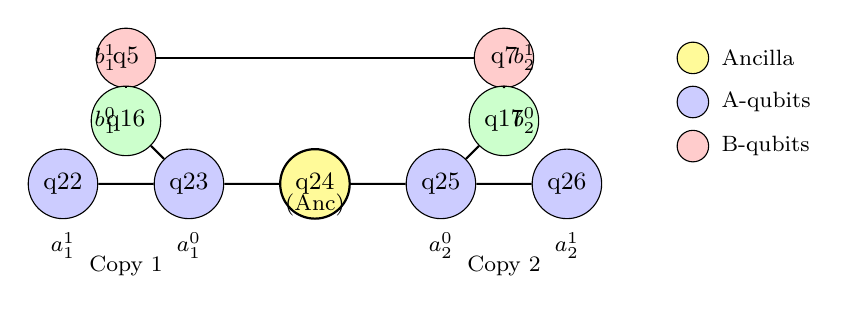
\begin{tikzpicture}[scale=0.8, every node/.style={font=\small}]
    % Top row - B qubits (bridges)
    \node[circle, draw, fill=red!20, minimum size=6mm] (q5) at (0, 3) {q5};
    \node[circle, draw, fill=red!20, minimum size=6mm] (q7) at (6, 3) {q7};
    \draw[thick] (q5) -- (q7);

    % Bridge qubits
    \node[circle, draw, fill=green!20, minimum size=6mm] (q16) at (0, 2) {q16};
    \node[circle, draw, fill=green!20, minimum size=6mm] (q17) at (6, 2) {q17};
    \draw[thick] (q5) -- (q16);
    \draw[thick] (q7) -- (q17);

    % Main row with ancilla
    \node[circle, draw, fill=blue!20, minimum size=6mm] (q22) at (-1, 1) {q22};
    \node[circle, draw, fill=blue!20, minimum size=6mm] (q23) at (1, 1) {q23};
    \node[circle, draw, fill=yellow!40, minimum size=8mm, thick] (q24) at (3, 1) {q24};
    \node[circle, draw, fill=blue!20, minimum size=6mm] (q25) at (5, 1) {q25};
    \node[circle, draw, fill=blue!20, minimum size=6mm] (q26) at (7, 1) {q26};

    \draw[thick] (q22) -- (q23) -- (q24) -- (q25) -- (q26);
    \draw[thick] (q16) -- (q23);
    \draw[thick] (q17) -- (q25);

    % Labels
    \node[below] at (q24) {\footnotesize (Anc)};
    \node[below=0.5cm] at (q22) {\footnotesize $a_1^1$};
    \node[below=0.5cm] at (q23) {\footnotesize $a_1^0$};
    \node[below=0.5cm] at (q25) {\footnotesize $a_2^0$};
    \node[below=0.5cm] at (q26) {\footnotesize $a_2^1$};

    \node[left] at (q16) {\footnotesize $b_1^0$};
    \node[left] at (q5) {\footnotesize $b_1^1$};
    \node[right] at (q17) {\footnotesize $b_2^0$};
    \node[right] at (q7) {\footnotesize $b_2^1$};

    % Copy labels
    \node at (0, -0.3) {\footnotesize Copy 1};
    \node at (6, -0.3) {\footnotesize Copy 2};

    % Legend
    \node[circle, draw, fill=yellow!40, minimum size=4mm] at (9, 3) {};
    \node[right, font=\footnotesize] at (9.3, 3) {Ancilla};
    \node[circle, draw, fill=blue!20, minimum size=4mm] at (9, 2.3) {};
    \node[right, font=\footnotesize] at (9.3, 2.3) {A-qubits};
    \node[circle, draw, fill=red!20, minimum size=4mm] at (9, 1.6) {};
    \node[right, font=\footnotesize] at (9.3, 1.6) {B-qubits};
\end{tikzpicture}
\end{center}

\textbf{Physical qubit assignment:}
\begin{center}
\begin{tabular}{|c|c|l||c|c|l|}
\hline
\multicolumn{3}{|c||}{Copy 1} & \multicolumn{3}{c|}{Copy 2} \\
\hline
Wire & Qubit & Role & Wire & Qubit & Role \\
\hline
1 & q23 & $a_1^0$ & 5 & q25 & $a_2^0$ \\
2 & q22 & $a_1^1$ & 6 & q26 & $a_2^1$ \\
3 & q16 & $b_1^0$ & 7 & q17 & $b_2^0$ \\
4 & q5 & $b_1^1$ & 8 & q7 & $b_2^1$ \\
\hline
\multicolumn{6}{|c|}{Ancilla: wire 0 $\to$ q24 (degree-3, central)} \\
\hline
\end{tabular}
\end{center}

\textbf{SWAP routing:}
\begin{itemize}
    \item SWAP$(1,5)$: q23 $\leftrightarrow$ q25 via q24 — \textbf{1 hop each}
    \item SWAP$(2,6)$: q22 $\leftrightarrow$ q26 via q23, q24, q25 — \textbf{2 hops each}
    \item SWAP$(3,7)$: q16 $\leftrightarrow$ q17 via q24 — \textbf{2 hops each}
    \item SWAP$(4,8)$: q5 $\leftrightarrow$ q7 via q16, q24, q17 — \textbf{3 hops each}
\end{itemize}

\textbf{Estimated overhead:} $\sim$8--12 routing SWAPs, $\sim$60--90 total CNOTs

\subsubsection{$S_4$ Mapping (17 qubits)}

\textbf{Strategy:} Arrange copies to minimize cross-SWAP distances. The critical swaps are $B_1 \leftrightarrow B_4$ and $B_2 \leftrightarrow B_3$ which connect non-adjacent copies.

\textbf{Optimized layout:} Place $B_1$ adjacent to $B_4$, and $B_2$ adjacent to $B_3$:

\begin{center}
\textbf{$S_4$ Optimized Topology Layout}
\vspace{0.3cm}

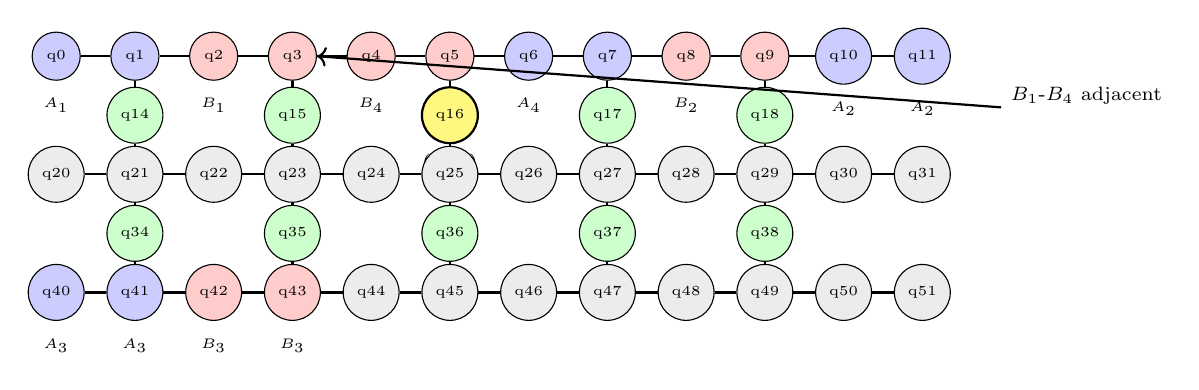
\begin{tikzpicture}[scale=0.5, every node/.style={font=\tiny}]
    % Row 0 - main qubits with role labels
    \foreach \i/\role/\col in {0/$A_1$/blue!20, 1/$A_1$/blue!20, 2/$B_1$/red!20, 3/$B_1$/red!20,
                               4/$B_4$/red!20, 5/$B_4$/red!20, 6/$A_4$/blue!20, 7/$A_4$/blue!20,
                               8/$B_2$/red!20, 9/$B_2$/red!20, 10/$A_2$/blue!20, 11/$A_2$/blue!20} {
        \node[circle, draw, fill=\col, minimum size=5mm] (r0q\i) at (\i*2.0, 6) {q\i};
        \node[below=1mm, font=\tiny] at (r0q\i.south) {\role};
    }
    % Horizontal edges Row 0
    \foreach \i in {0,...,10} {
        \pgfmathtruncatemacro{\j}{\i+1}
        \draw[thick] (r0q\i) -- (r0q\j);
    }

    % Bridge qubits between Row 0 and Row 1
    \node[circle, draw, fill=green!20, minimum size=5mm] (q14) at (1*2.0, 4.5) {q14};
    \node[circle, draw, fill=green!20, minimum size=5mm] (q15) at (3*2.0, 4.5) {q15};
    \node[circle, draw, fill=yellow!50, minimum size=7mm, thick] (q16) at (5*2.0, 4.5) {q16};
    \node[circle, draw, fill=green!20, minimum size=5mm] (q17) at (7*2.0, 4.5) {q17};
    \node[circle, draw, fill=green!20, minimum size=5mm] (q18) at (9*2.0, 4.5) {q18};

    \node[below=0mm] at (q16.south) {\scriptsize (Anc)};

    \draw[thick] (r0q1) -- (q14); \draw[thick] (r0q3) -- (q15);
    \draw[thick] (r0q5) -- (q16); \draw[thick] (r0q7) -- (q17);
    \draw[thick] (r0q9) -- (q18);

    % Row 1
    \foreach \i in {0,...,11} {
        \pgfmathtruncatemacro{\q}{\i+20}
        \node[circle, draw, fill=gray!15, minimum size=5mm] (r1q\q) at (\i*2.0, 3) {q\q};
    }
    \foreach \i in {20,...,30} {
        \pgfmathtruncatemacro{\j}{\i+1}
        \draw[thick] (r1q\i) -- (r1q\j);
    }
    \draw[thick] (q14) -- (r1q21); \draw[thick] (q15) -- (r1q23);
    \draw[thick] (q16) -- (r1q25); \draw[thick] (q17) -- (r1q27);
    \draw[thick] (q18) -- (r1q29);

    % Bridge qubits between Row 1 and Row 2
    \node[circle, draw, fill=green!20, minimum size=5mm] (q34) at (1*2.0, 1.5) {q34};
    \node[circle, draw, fill=green!20, minimum size=5mm] (q35) at (3*2.0, 1.5) {q35};
    \node[circle, draw, fill=green!20, minimum size=5mm] (q36) at (5*2.0, 1.5) {q36};
    \node[circle, draw, fill=green!20, minimum size=5mm] (q37) at (7*2.0, 1.5) {q37};
    \node[circle, draw, fill=green!20, minimum size=5mm] (q38) at (9*2.0, 1.5) {q38};

    \draw[thick] (r1q21) -- (q34); \draw[thick] (r1q23) -- (q35);
    \draw[thick] (r1q25) -- (q36); \draw[thick] (r1q27) -- (q37);
    \draw[thick] (r1q29) -- (q38);

    % Row 2 - with role labels
    \foreach \i/\role/\col in {0/$A_3$/blue!20, 1/$A_3$/blue!20, 2/$B_3$/red!20, 3/$B_3$/red!20,
                               4//gray!15, 5//gray!15, 6//gray!15, 7//gray!15,
                               8//gray!15, 9//gray!15, 10//gray!15, 11//gray!15} {
        \pgfmathtruncatemacro{\q}{\i+40}
        \node[circle, draw, fill=\col, minimum size=5mm] (r2q\q) at (\i*2.0, 0) {q\q};
        \ifx\role\empty\else
            \node[below=1mm, font=\tiny] at (r2q\q.south) {\role};
        \fi
    }
    \foreach \i in {40,...,50} {
        \pgfmathtruncatemacro{\j}{\i+1}
        \draw[thick] (r2q\i) -- (r2q\j);
    }
    \draw[thick] (q34) -- (r2q41); \draw[thick] (q35) -- (r2q43);
    \draw[thick] (q36) -- (r2q45); \draw[thick] (q37) -- (r2q47);
    \draw[thick] (q38) -- (r2q49);

    % Legend
    \node[right, font=\scriptsize] at (24, 5) {$B_1$-$B_4$ adjacent};
    \draw[->, thick] (24, 4.7) -- (r0q3.east);
\end{tikzpicture}
\end{center}

\textbf{Physical qubit assignment:}
\begin{center}
\begin{tabular}{|c|c|c||c|c|c|}
\hline
Wire & Qubit & Role & Wire & Qubit & Role \\
\hline
0 & q16 & Ancilla & & & \\
\hline
1 & q0 & $a_1^0$ & 9 & q40 & $a_3^0$ \\
2 & q1 & $a_1^1$ & 10 & q41 & $a_3^1$ \\
3 & q2 & $b_1^0$ & 11 & q42 & $b_3^0$ \\
4 & q3 & $b_1^1$ & 12 & q43 & $b_3^1$ \\
\hline
5 & q10 & $a_2^0$ & 13 & q6 & $a_4^0$ \\
6 & q11 & $a_2^1$ & 14 & q7 & $a_4^1$ \\
7 & q8 & $b_2^0$ & 15 & q4 & $b_4^0$ \\
8 & q9 & $b_2^1$ & 16 & q5 & $b_4^1$ \\
\hline
\end{tabular}
\end{center}

\textbf{Key advantage:} $B_1$(q2,q3) is adjacent to $B_4$(q4,q5), minimizing the cross-swap distance.

\textbf{Estimated overhead:} $\sim$20--30 routing SWAPs, $\sim$160--240 total CNOTs

\subsubsection{$S_6$ Mapping (25 qubits)}

\textbf{Strategy:} The critical swap $B_1 \leftrightarrow B_6$ spans all 6 copies. Use a folded/circular arrangement to place $B_1$ near $B_6$.

\begin{center}
\textbf{$S_6$ Folded Topology Layout}
\vspace{0.3cm}

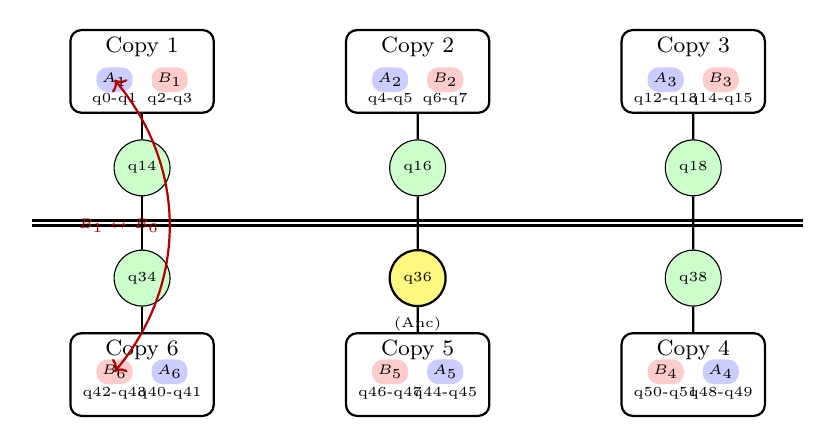
\begin{tikzpicture}[scale=0.7, every node/.style={font=\small}]
    % Top row boxes (Copies 1, 2, 3)
    \foreach \c/\x/\al/\bl/\aq/\bq in {1/0/A_1/B_1/{q0-q1}/{q2-q3},
                                        2/5/A_2/B_2/{q4-q5}/{q6-q7},
                                        3/10/A_3/B_3/{q12-q13}/{q14-q15}} {
        \draw[thick, rounded corners] (\x-1.3, 4) rectangle (\x+1.3, 5.5);
        \node at (\x, 5.2) {\footnotesize Copy \c};
        \node[fill=blue!20, rounded corners, inner sep=2pt] at (\x-0.5, 4.6) {\tiny $\al$};
        \node[fill=red!20, rounded corners, inner sep=2pt] at (\x+0.5, 4.6) {\tiny $\bl$};
        \node[font=\tiny] at (\x-0.5, 4.25) {\aq};
        \node[font=\tiny] at (\x+0.5, 4.25) {\bq};
    }

    % Bridge qubits (top)
    \node[circle, draw, fill=green!20, minimum size=5mm, font=\tiny] (br1) at (0, 3) {q14};
    \node[circle, draw, fill=green!20, minimum size=5mm, font=\tiny] (br2) at (5, 3) {q16};
    \node[circle, draw, fill=green!20, minimum size=5mm, font=\tiny] (br3) at (10, 3) {q18};

    \draw[thick] (0, 4) -- (br1);
    \draw[thick] (5, 4) -- (br2);
    \draw[thick] (10, 4) -- (br3);

    % Central horizontal line (main bus)
    \draw[very thick, double] (-2, 2) -- (12, 2);

    % Bridge qubits (bottom) with ancilla
    \node[circle, draw, fill=green!20, minimum size=5mm, font=\tiny] (bb1) at (0, 1) {q34};
    \node[circle, draw, fill=yellow!50, minimum size=7mm, font=\tiny, thick] (anc) at (5, 1) {q36};
    \node[below=0mm, font=\tiny] at (anc.south) {(Anc)};
    \node[circle, draw, fill=green!20, minimum size=5mm, font=\tiny] (bb3) at (10, 1) {q38};

    \draw[thick] (br1) -- (0, 2) -- (bb1);
    \draw[thick] (br2) -- (5, 2) -- (anc);
    \draw[thick] (br3) -- (10, 2) -- (bb3);

    % Bottom row boxes (Copies 6, 5, 4) - note reversed order
    \foreach \c/\x/\al/\bl/\aq/\bq in {6/0/B_6/A_6/{q42-q43}/{q40-q41},
                                        5/5/B_5/A_5/{q46-q47}/{q44-q45},
                                        4/10/B_4/A_4/{q50-q51}/{q48-q49}} {
        \draw[thick, rounded corners] (\x-1.3, -1.5) rectangle (\x+1.3, 0);
        \node at (\x, -0.3) {\footnotesize Copy \c};
        \node[fill=red!20, rounded corners, inner sep=2pt] at (\x-0.5, -0.7) {\tiny $\al$};
        \node[fill=blue!20, rounded corners, inner sep=2pt] at (\x+0.5, -0.7) {\tiny $\bl$};
        \node[font=\tiny] at (\x-0.5, -1.1) {\aq};
        \node[font=\tiny] at (\x+0.5, -1.1) {\bq};
    }

    \draw[thick] (bb1) -- (0, 0);
    \draw[thick] (anc) -- (5, 0);
    \draw[thick] (bb3) -- (10, 0);

    % Annotation
    \draw[<->, thick, red!70!black] (-0.5, 4.6) to[bend left=40] node[midway, left, font=\tiny] {$B_1 \leftrightarrow B_6$} (-0.5, -0.7);
\end{tikzpicture}

\smallskip
\textit{Key: $B_1$(q2,q3) is now close to $B_6$(q42,q43) via bridge path.}
\end{center}

\textbf{Physical qubit assignment:}
\begin{center}
\begin{tabular}{|c|c|c|c||c|c|c|c|}
\hline
Copy & Wire & Qubit & Role & Copy & Wire & Qubit & Role \\
\hline
1 & 1 & q0 & $a_1^0$ & 4 & 13 & q48 & $a_4^0$ \\
1 & 2 & q1 & $a_1^1$ & 4 & 14 & q49 & $a_4^1$ \\
1 & 3 & q2 & $b_1^0$ & 4 & 15 & q50 & $b_4^0$ \\
1 & 4 & q3 & $b_1^1$ & 4 & 16 & q51 & $b_4^1$ \\
\hline
2 & 5 & q4 & $a_2^0$ & 5 & 17 & q44 & $a_5^0$ \\
2 & 6 & q5 & $a_2^1$ & 5 & 18 & q45 & $a_5^1$ \\
2 & 7 & q6 & $b_2^0$ & 5 & 19 & q46 & $b_5^0$ \\
2 & 8 & q7 & $b_2^1$ & 5 & 20 & q47 & $b_5^1$ \\
\hline
3 & 9 & q12 & $a_3^0$ & 6 & 21 & q40 & $a_6^0$ \\
3 & 10 & q13 & $a_3^1$ & 6 & 22 & q41 & $a_6^1$ \\
3 & 11 & q14 & $b_3^0$ & 6 & 23 & q42 & $b_6^0$ \\
3 & 12 & q15 & $b_3^1$ & 6 & 24 & q43 & $b_6^1$ \\
\hline
\multicolumn{8}{|c|}{Ancilla: wire 0 $\to$ q36 (central bridge)} \\
\hline
\end{tabular}
\end{center}

\textbf{Critical path:} $B_1 \leftrightarrow B_6$ = q2,q3 $\leftrightarrow$ q42,q43 via bridges q14, q34 — approximately 6 hops.

\textbf{Estimated overhead:} $\sim$40--60 routing SWAPs, $\sim$320--480 total CNOTs

\subsubsection{$T_4$ Mapping (17 qubits)}

$T_4$ uses \textbf{cyclic} permutations, which benefit from \textbf{linear} qubit arrangement:
\begin{align*}
(\pi_4^{-1})_A &: A_1 \to A_4 \to A_3 \to A_2 \to A_1 \quad \text{(shift right)} \\
(\pi_4)_B &: B_1 \to B_2 \to B_3 \to B_4 \to B_1 \quad \text{(shift left)}
\end{align*}

\textbf{Optimal layout:} Place $A_1$--$A_2$--$A_3$--$A_4$ and $B_1$--$B_2$--$B_3$--$B_4$ in linear chains:

\begin{center}
\textbf{$T_4$ Linear Topology Layout}
\vspace{0.3cm}

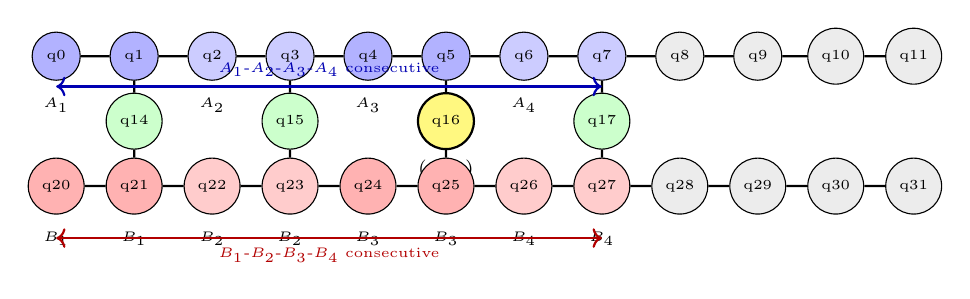
\begin{tikzpicture}[scale=0.55, every node/.style={font=\tiny}]
    % Row 0 - A qubits (linear arrangement A1-A2-A3-A4)
    \foreach \i/\role/\col in {0/$A_1$/blue!30, 1/$A_1$/blue!30, 2/$A_2$/blue!20, 3/$A_2$/blue!20,
                               4/$A_3$/blue!30, 5/$A_3$/blue!30, 6/$A_4$/blue!20, 7/$A_4$/blue!20,
                               8//gray!15, 9//gray!15, 10//gray!15, 11//gray!15} {
        \node[circle, draw, fill=\col, minimum size=5mm] (r0q\i) at (\i*1.8, 4) {q\i};
        \ifx\role\empty\else
            \node[below=1mm] at (r0q\i.south) {\role};
        \fi
    }
    \foreach \i in {0,...,10} {
        \pgfmathtruncatemacro{\j}{\i+1}
        \draw[thick] (r0q\i) -- (r0q\j);
    }

    % Bridge qubits with ancilla
    \node[circle, draw, fill=green!20, minimum size=5mm] (q14) at (1*1.8, 2.5) {q14};
    \node[circle, draw, fill=green!20, minimum size=5mm] (q15) at (3*1.8, 2.5) {q15};
    \node[circle, draw, fill=yellow!50, minimum size=7mm, thick] (q16) at (5*1.8, 2.5) {q16};
    \node[circle, draw, fill=green!20, minimum size=5mm] (q17) at (7*1.8, 2.5) {q17};

    \node[below=0mm] at (q16.south) {\scriptsize (Anc)};

    \draw[thick] (r0q1) -- (q14); \draw[thick] (r0q3) -- (q15);
    \draw[thick] (r0q5) -- (q16); \draw[thick] (r0q7) -- (q17);

    % Row 1 - B qubits (linear arrangement B1-B2-B3-B4)
    \foreach \i/\role/\col in {0/$B_1$/red!30, 1/$B_1$/red!30, 2/$B_2$/red!20, 3/$B_2$/red!20,
                               4/$B_3$/red!30, 5/$B_3$/red!30, 6/$B_4$/red!20, 7/$B_4$/red!20,
                               8//gray!15, 9//gray!15, 10//gray!15, 11//gray!15} {
        \pgfmathtruncatemacro{\q}{\i+20}
        \node[circle, draw, fill=\col, minimum size=5mm] (r1q\q) at (\i*1.8, 1) {q\q};
        \ifx\role\empty\else
            \node[below=1mm] at (r1q\q.south) {\role};
        \fi
    }
    \foreach \i in {20,...,30} {
        \pgfmathtruncatemacro{\j}{\i+1}
        \draw[thick] (r1q\i) -- (r1q\j);
    }

    \draw[thick] (q14) -- (r1q21); \draw[thick] (q15) -- (r1q23);
    \draw[thick] (q16) -- (r1q25); \draw[thick] (q17) -- (r1q27);

    % Annotations showing linear arrangement
    \draw[<->, thick, blue!70!black] (0, 3.3) -- (12.6, 3.3) node[midway, above, font=\tiny] {$A_1$-$A_2$-$A_3$-$A_4$ consecutive};
    \draw[<->, thick, red!70!black] (0, -0.2) -- (12.6, -0.2) node[midway, below, font=\tiny] {$B_1$-$B_2$-$B_3$-$B_4$ consecutive};
\end{tikzpicture}

\smallskip
\textit{Linear arrangement enables minimal routing for cyclic permutations.}
\end{center}

\textbf{Cyclic SWAP decomposition:}
\begin{itemize}
    \item $(\pi_4^{-1})_A$: SWAP$(A_3,A_4)$, then SWAP$(A_2,A_3)$, then SWAP$(A_1,A_2)$
    \item Each SWAP is between adjacent qutrits — \textbf{no routing needed!}
\end{itemize}

\textbf{Estimated overhead:} $\sim$12--20 routing SWAPs, $\sim$140--200 total CNOTs (better than $S_4$!)

\subsubsection{Resource Summary with Topology Overhead}

\begin{center}
\begin{tabular}{|c|c|c|c|c|c|}
\hline
\textbf{Circuit} & \textbf{Qubits} & \textbf{Logical c-SWAPs} & \textbf{Routing SWAPs} & \textbf{Total CNOTs} & \textbf{Depth} \\
\hline
$S_2$ & 9 & 4 & $\sim$8--12 & $\sim$60--90 & $\sim$40 \\
$S_4$ & 17 & 8 & $\sim$20--30 & $\sim$160--240 & $\sim$80 \\
$S_6$ & 25 & 12 & $\sim$40--60 & $\sim$320--480 & $\sim$150 \\
$T_4$ & 17 & 12 & $\sim$12--20 & $\sim$140--200 & $\sim$70 \\
\hline
\end{tabular}
\end{center}

\textbf{Practical recommendations:}
\begin{enumerate}
    \item Select qubits in a connected 2--3 row region with low error rates
    \item Place ancilla at a central degree-3 qubit
    \item For $S_k$: Group qutrit pairs that will be swapped close together
    \item For $T_k$: Use linear arrangement for the cyclic permutation direction
    \item Compile with topology-aware tools (e.g., \texttt{qiskit.transpile} with \texttt{optimization\_level=3})
    \item Use measurement error mitigation (M3 or mthree package)
\end{enumerate}

\subsection{Circuit Validation}

The circuits have been numerically validated by computing:
\begin{enumerate}
    \item $S_k$ directly from the singular values of $R(\rho)$
    \item $S_k$ from the matrix formula $\Tr[(R^\dagger R)^{k/2}]$
    \item $S_k$ from the permutation formula $\Tr[\rho^{\otimes 2k} (\Pi_A^{(2k)} \otimes \Pi_B^{(2k)})]$
\end{enumerate}

All three methods give identical results to machine precision, confirming that the permutation operators are correct:

\begin{center}
\begin{tabular}{|c|c|c|c|}
\hline
\textbf{Moment} & \textbf{SVD} & \textbf{Matrix} & \textbf{Permutation} \\
\hline
$S_2$ & 0.4853561627 & 0.4853561627 & 0.4853561627 \\
$S_4$ & 0.1817684988 & 0.1817684988 & 0.1817684988 \\
$S_6$ & 0.0760882278 & 0.0760882278 & 0.0760882278 \\
\hline
\end{tabular}
\end{center}

\textbf{Validation confirms:}
\begin{itemize}
    \item $\Pi_A^{(4)} = \SWAP_{1,2} \SWAP_{3,4}$ (pairwise swaps on $A$) is correct
    \item $\Pi_B^{(4)} = \SWAP_{1,4} \SWAP_{2,3}$ (cross swaps on $B$) is correct
    \item The Hadamard test yields $S_k = 2P(0) - 1$
\end{itemize}

\subsection{Resource Summary}

\begin{table}[ht]
\centering
\begin{tabular}{|c|c|c|c|c|}
\hline
\textbf{Moment} & \textbf{Copies} & \textbf{Ancilla} & \textbf{c-SWAPs} & \textbf{Formula} \\
\hline
$S_2$ & 2 & 1 & 2 & $\SWAP_A \otimes \SWAP_B$ \\
$S_4$ & 4 & 1 & 4 & $\SWAP_{12}\SWAP_{34} \otimes \SWAP_{14}\SWAP_{23}$ \\
$S_6$ & 6 & 1 & 6 & $\SWAP_{12}\SWAP_{34}\SWAP_{56} \otimes \SWAP_{16}\SWAP_{23}\SWAP_{45}$ \\
$S_{2k}$ & $2k$ & 1 & $2k$ & General formula \\
\hline
\end{tabular}
\caption{Resource requirements for measuring realignment moments}
\end{table}

\section{Chirality Observables: $C_{2k} = T_{2k} - S_{2k}$}

The quantity $C_{2k} = T_{2k} - S_{2k}$ measures the difference between partial transpose moments and realignment moments. It can be expressed as the expectation of a \textbf{chirality operator}.

\subsection{Multi-Copy Observable Representations}

Both moments have permutation representations on $2k$ copies:
\begin{align}
T_{2k} &= \Tr[\rho^{\otimes 2k} \cdot (\pi_{2k}^{-1})_A \otimes (\pi_{2k})_B] \\
S_{2k} &= \Tr[\rho^{\otimes 2k} \cdot \Pi_A^{(2k)} \otimes \Pi_B^{(2k)}]
\end{align}

\subsection{The Chirality Operator}

\begin{definition}[Chirality Operator]
The chirality operator on $2k$ copies is:
\begin{equation}
\boxed{\chi_{2k} = (\pi_{2k}^{-1})_A \otimes (\pi_{2k})_B - \Pi_A^{(2k)} \otimes \Pi_B^{(2k)}}
\end{equation}
and the chirality observable is:
\begin{equation}
C_{2k} = \Tr[\rho^{\otimes 2k} \cdot \chi_{2k}]
\end{equation}
\end{definition}

\subsection{Physical Interpretation}

The two terms in $\chi_{2k}$ have fundamentally different symmetry properties:

\begin{center}
\begin{tabular}{|l|c|c|}
\hline
\textbf{Property} & \textbf{PT term} & \textbf{Realignment term} \\
\hline
A-permutation & $\pi_{2k}^{-1}$ (inverse cyclic) & Pairwise SWAPs \\
B-permutation & $\pi_{2k}$ (cyclic) & Cross SWAPs \\
Chirality & Opposite on A vs B & Achiral (self-inverse) \\
Order & $2k$ & 2 \\
\hline
\end{tabular}
\end{center}

\textbf{Chirality interpretation:}
\begin{itemize}
    \item The PT term uses cyclic permutations rotating in \textbf{opposite directions} on A and B
    \item The realignment term uses products of transpositions (SWAPs), which are \textbf{achiral}
    \item $C_{2k}$ measures the difference between these ``chiral'' and ``achiral'' correlation structures
\end{itemize}

\subsection{Explicit Formulas}

\subsubsection{$C_2 = T_2 - S_2$ (2 copies)}

For 2 copies, $\pi_2 = (1\ 2)$ is a transposition, so $\pi_2^{-1} = \pi_2$:
\begin{align}
T_2 &: (\text{SWAP})_A \otimes (\text{SWAP})_B \\
S_2 &: (\text{SWAP})_A \otimes (\text{SWAP})_B
\end{align}

Therefore:
\begin{equation}
\boxed{C_2 = T_2 - S_2 = 0 \quad \text{(identically for all states)}}
\end{equation}

This confirms the identity $\Tr[(\rho^{T_A})^2] = \Tr[\rho^2] = \Tr[R^\dagger R]$.

\subsubsection{$C_4 = T_4 - S_4$ (4 copies)}

\begin{align}
T_4 &: \underbrace{(4\ 3\ 2\ 1)}_{\text{inv. 4-cycle}}\!{}_A \otimes \underbrace{(1\ 2\ 3\ 4)}_{\text{4-cycle}}\!{}_B \\[5pt]
S_4 &: \underbrace{(1\leftrightarrow 2)(3\leftrightarrow 4)}_{\text{pairwise}}\!{}_A \otimes \underbrace{(1\leftrightarrow 4)(2\leftrightarrow 3)}_{\text{cross}}\!{}_B
\end{align}

The chirality operator:
\begin{equation}
\chi_4 = (4\ 3\ 2\ 1)_A \otimes (1\ 2\ 3\ 4)_B - (1\ 2)(3\ 4)_A \otimes (1\ 4)(2\ 3)_B
\end{equation}

\subsubsection{$C_6 = T_6 - S_6$ (6 copies)}

\begin{align}
T_6 &: (6\ 5\ 4\ 3\ 2\ 1)_A \otimes (1\ 2\ 3\ 4\ 5\ 6)_B \\[5pt]
S_6 &: (1\ 2)(3\ 4)(5\ 6)_A \otimes (1\ 6)(2\ 3)(4\ 5)_B
\end{align}

\subsection{Quantum Circuits for $C_{2k}$}

To measure $C_{2k}$, we need circuits for both $T_{2k}$ and $S_{2k}$.

\subsubsection{Circuit for $T_4$ (PT moment)}

The permutation $(4\ 3\ 2\ 1)_A \otimes (1\ 2\ 3\ 4)_B$ requires controlled cyclic shifts:

\begin{center}
\begin{quantikz}[row sep=0.3cm, column sep=0.4cm]
\lstick{$\ket{0}$} & \gate{H} & \ctrl{1} & \ctrl{5} & \gate{H} & \meter{} \\
\lstick{$A_1$} & \qw & \gate[4]{\pi_4^{-1}} & \qw & \qw & \qw \\
\lstick{$A_2$} & \qw & \qw & \qw & \qw & \qw \\
\lstick{$A_3$} & \qw & \qw & \qw & \qw & \qw \\
\lstick{$A_4$} & \qw & \qw & \qw & \qw & \qw \\
\lstick{$B_1$} & \qw & \qw & \gate[4]{\pi_4} & \qw & \qw \\
\lstick{$B_2$} & \qw & \qw & \qw & \qw & \qw \\
\lstick{$B_3$} & \qw & \qw & \qw & \qw & \qw \\
\lstick{$B_4$} & \qw & \qw & \qw & \qw & \qw
\end{quantikz}
\end{center}

where $\pi_4$ is the 4-cycle $(1\ 2\ 3\ 4)$ and $\pi_4^{-1} = (4\ 3\ 2\ 1)$.

\subsubsection{Circuit for $S_4$ (Realignment moment)}

As derived earlier, uses pairwise and cross SWAPs:

\begin{center}
\begin{quantikz}[row sep=0.35cm, column sep=0.5cm]
\lstick{Anc.} & \gate{H} & \ctrl{1} & \ctrl{3} & \ctrl{6} & \ctrl{5} & \gate{H} & \meter{} \\
\lstick{$A_1$} & \qw & \swap{1} & \qw      & \qw      & \qw      & \qw & \qw \\
\lstick{$A_2$} & \qw & \targX{} & \qw      & \qw      & \qw      & \qw & \qw \\
\lstick{$A_3$} & \qw & \qw      & \swap{1} & \qw      & \qw      & \qw & \qw \\
\lstick{$A_4$} & \qw & \qw      & \targX{} & \qw      & \qw      & \qw & \qw \\
\lstick{$B_1$} & \qw & \qw      & \qw      & \qw      & \swap{3} & \qw & \qw \\
\lstick{$B_2$} & \qw & \qw      & \qw      & \swap{1} & \qw      & \qw & \qw \\
\lstick{$B_3$} & \qw & \qw      & \qw      & \targX{} & \qw      & \qw & \qw \\
\lstick{$B_4$} & \qw & \qw      & \qw      & \qw      & \targX{} & \qw & \qw
\end{quantikz}
\end{center}

\subsubsection{Computing $C_4$}

From the Hadamard test:
\begin{align}
T_4 &= 2P_{T_4}(0) - 1 \\
S_4 &= 2P_{S_4}(0) - 1
\end{align}

Therefore:
\begin{equation}
C_4 = T_4 - S_4 = 2[P_{T_4}(0) - P_{S_4}(0)]
\end{equation}

\subsection{Numerical Values}

\begin{table}[ht]
\centering
\begin{tabular}{|l|c|c|c|}
\hline
\textbf{State} & $C_2$ & $C_4$ & $C_6$ \\
\hline
Maximally mixed $\mathbb{1}/4$ & 0 & $-0.047$ & --- \\
Pure product $|0\rangle \otimes |+\rangle$ & 0 & 0 & 0 \\
Bell state $|\Phi^+\rangle$ & 0 & 0 & 0 \\
Werner $W(0.5)$ & 0 & $-0.015$ & --- \\
Random entangled & 0 & $-0.014$ & $-0.010$ \\
\hline
\end{tabular}
\caption{$C_{2k}$ values for various states. Note $C_2 = 0$ identically.}
\end{table}

\subsection{Key Observations}

\begin{enumerate}
    \item $C_2 = 0$ for \textbf{all} bipartite states (identity)
    \item For pure states (product or entangled): $C_{2k} = 0$ for all $k$
    \item For mixed states: $C_{2k} \neq 0$ in general, with $C_{2k} \leq 0$ typically
    \item The chirality difference measures how the state's correlations align with cyclic vs.\ reflective permutation structures
\end{enumerate}

\section{The Hermitian Trace Invariants $G_k$ and Combined Witnesses}

While $S_k = \Tr[(R^\dagger R)^{k/2}]$ captures information about the singular values of the realignment matrix, additional entanglement signatures are encoded in the \textbf{trace} of powers of $R$ itself.

\subsection{Definition of $G_k$ and $K_k$}

The trace of $R^k$ is generally complex. We decompose it into real and imaginary parts:

\begin{definition}[Hermitian Trace Invariants]
For the realignment matrix $R(\rho)$, define:
\begin{align}
G_k &= \Re\left(\Tr[R^k]\right) = \frac{\Tr[R^k] + \Tr[(R^k)^\dagger]}{2} \label{eq:Gk_def} \\
K_k &= \Im\left(\Tr[R^k]\right) = \frac{\Tr[R^k] - \Tr[(R^k)^\dagger]}{2i} \label{eq:Kk_def}
\end{align}
so that $\Tr[R^k] = G_k + i K_k$.
\end{definition}

\textbf{Key properties:}
\begin{itemize}
    \item $G_k$ measures the \textbf{Hermitian part} of $\Tr[R^k]$, related to the sum of real parts of eigenvalues of $R^k$
    \item $K_k$ measures the \textbf{anti-Hermitian part}, related to the sum of imaginary parts
    \item For states with real density matrices (in the computational basis), $K_k = 0$
    \item The ratio $G_k/S_k \in [-1, 1]$ measures how ``Hermitian'' the realignment matrix behaves
\end{itemize}

\subsection{Relationship Between $S_k$ and $G_k$}

The invariants $S_k$ and $G_k$ are related but distinct:
\begin{itemize}
    \item $S_k = \sum_i \sigma_i^k$ where $\{\sigma_i\}$ are the \textbf{singular values} of $R$
    \item $G_k = \Re\left(\sum_j \lambda_j^k\right)$ where $\{\lambda_j\}$ are the \textbf{eigenvalues} of $R$
\end{itemize}

For a Hermitian matrix, $\lambda_j = \pm\sigma_j$ (eigenvalues equal signed singular values), so $G_k = S_k$ when $k$ is even. The deviation $\Delta_k = S_k - G_k \geq 0$ measures the non-Hermiticity of $R$.

\begin{proposition}
For any quantum state $\rho_{AB}$:
\begin{equation}
\frac{G_k}{S_k} \in [-1, 1]
\end{equation}
with $G_k/S_k = 1$ if and only if $R(\rho)$ has only non-negative real eigenvalues.
\end{proposition}

\subsection{Physical Interpretation}

Bound entangled states often exhibit a characteristic feature: their realignment matrices are ``nearly Hermitian,'' manifesting as:
\begin{equation}
\frac{G_2}{S_2} \to 1 \quad \text{(high Hermitianity)}
\end{equation}

This can be understood intuitively: bound entangled states occupy a constrained region of state space (PPT yet entangled), and this constraint tends to produce realignment matrices with more structured eigenvalue distributions.

\subsection{Combined Entanglement Witness}

The individual invariants $S_k$ and $G_k$ have overlapping distributions between separable and bound entangled states. However, \textbf{combining} them yields a powerful witness with zero false positives.

\begin{theorem}[Combined $S_k$-$G_k$ Witness]
For $3 \times 3$ systems, the criterion:
\begin{equation}
\boxed{\frac{G_2}{S_2} > 0.85 \quad \text{AND} \quad \frac{S_2 \cdot S_6}{S_4^2} > 1.25}
\label{eq:combined_witness}
\end{equation}
detects entanglement with:
\begin{itemize}
    \item \textbf{Zero false positives} on 90,000 tested separable states
    \item \textbf{78\% detection rate} on the Horodecki bound entangled family
\end{itemize}
\end{theorem}

\textbf{Interpretation:} This combined criterion identifies states that simultaneously:
\begin{enumerate}
    \item Have nearly Hermitian realignment matrices ($G_2/S_2 > 0.85$)
    \item Violate the Cauchy-Schwarz-type moment inequality ($S_2 S_6/S_4^2 > 1.25$)
\end{enumerate}

\subsection{Comparison of Witnesses}

\begin{center}
\begin{tabular}{|l|c|c|c|}
\hline
\textbf{Criterion} & \textbf{Threshold} & \textbf{FP Rate} & \textbf{Detection} \\
\hline
$S_2 S_6/S_4^2$ alone & $> 1.35$ & 0\% & $\sim$60\% \\
$G_2/S_2$ alone & $> 0.85$ & $>0$\% & --- \\
Combined (Eq.~\ref{eq:combined_witness}) & Both & 0\% & 78\% \\
\hline
\end{tabular}
\end{center}

The combined criterion achieves higher detection rates than $S_2 S_6/S_4^2 > 1.35$ alone by relaxing the moment ratio threshold (from 1.35 to 1.25) while adding the $G_2/S_2$ constraint to maintain zero false positives.

\subsection{Quantum Circuit for $G_2$}

We derive an explicit quantum circuit for measuring $G_2 = \Re(\Tr[R^2])$ using a Hadamard test on two copies of the state.

\subsubsection{Permutation Structure}

Using the realignment definition $R_{(ij),(\mu\nu)} = \rho_{i\mu,j\nu}$, we compute:
\begin{align}
\Tr[R^2] &= \sum_{i,j} [R^2]_{(ij),(ij)} = \sum_{i,j,\mu,\nu} R_{(ij),(\mu\nu)} R_{(\mu\nu),(ij)} \\
&= \sum_{i,j,\mu,\nu} \rho_{i\mu,j\nu} \cdot \rho_{\mu i, \nu j}
\end{align}

This contraction over two copies of $\rho$ corresponds to a specific permutation:

\begin{theorem}[$G_2$ Permutation Formula]
For a $d \times d$ bipartite system:
\begin{equation}
\boxed{G_2 = \Tr\left[\rho^{\otimes 2} \cdot \text{SWAP}_{A_1 \leftrightarrow B_2} \cdot \text{SWAP}_{B_1 \leftrightarrow A_2}\right]}
\end{equation}
where $A_i, B_i$ denote the $A$ and $B$ subsystems of copy $i$.
\end{theorem}

\textbf{Key difference from $S_2$:} The $S_2$ circuit uses ``parallel'' SWAPs ($A_1 \leftrightarrow A_2$ and $B_1 \leftrightarrow B_2$), while $G_2$ uses ``crossed'' SWAPs that exchange $A \leftrightarrow B$ between copies.

\subsubsection{Circuit Diagram}

For a $3 \times 3$ system with qutrits encoded in 2 qubits each:

\begin{center}
\textbf{Register layout:} Ancilla (1 qubit), $A_1, B_1, A_2, B_2$ (2 qubits each for qutrit encoding)

\vspace{0.5cm}
\begin{quantikz}[row sep=0.5cm, column sep=0.7cm]
\lstick{$\ket{0}$} & \gate{H} & \ctrl{2} & \ctrl{1} & \gate{H} & \meter{} \\
\lstick{$A_1$} & \qwbundle{2} & \qw & \swap{3} & \qw & \qw \\
\lstick{$B_1$} & \qwbundle{2} & \swap{1} & \qw & \qw & \qw \\
\lstick{$A_2$} & \qwbundle{2} & \targX{} & \qw & \qw & \qw \\
\lstick{$B_2$} & \qwbundle{2} & \qw & \targX{} & \qw & \qw
\end{quantikz}
\vspace{0.3cm}

\small
First c-SWAP: $B_1 \leftrightarrow A_2$ \quad|\quad Second c-SWAP: $A_1 \leftrightarrow B_2$
\end{center}

The circuit implements:
\begin{enumerate}
    \item \textbf{c-SWAP$(B_1, A_2)$}: Exchange $B$-subsystem of copy 1 with $A$-subsystem of copy 2
    \item \textbf{c-SWAP$(A_1, B_2)$}: Exchange $A$-subsystem of copy 1 with $B$-subsystem of copy 2
\end{enumerate}

\textbf{Result:} $G_2 = 2P(|0\rangle) - 1$

\subsubsection{Resource Comparison}

\begin{center}
\begin{tabular}{|l|c|c|c|}
\hline
\textbf{Observable} & \textbf{Permutation} & \textbf{c-SWAPs} & \textbf{CNOTs} \\
\hline
$S_2$ & $\text{SWAP}_{A_1 A_2} \otimes \text{SWAP}_{B_1 B_2}$ & 2 & $\sim$32 \\
$G_2$ & $\text{SWAP}_{A_1 B_2} \otimes \text{SWAP}_{B_1 A_2}$ & 2 & $\sim$32 \\
\hline
\end{tabular}
\end{center}

Both circuits have comparable gate complexity, but probe different matrix properties:
\begin{itemize}
    \item $S_2 = \sum_i \sigma_i^2$ (singular values)
    \item $G_2 = \Re(\sum_j \lambda_j^2)$ (eigenvalues)
\end{itemize}

\subsubsection{Physical Interpretation}

The ``crossed'' SWAP structure of the $G_2$ circuit probes how the realignment matrix $R$ mixes the $A$ and $B$ indices. For states with near-Hermitian $R$ (where eigenvalues are close to singular values), $G_2 \approx S_2$, yielding high $G_2/S_2$ ratios characteristic of bound entangled states.

\section{The Tiles Bound Entangled State}

The Tiles state is a paradigmatic example of bound entanglement---it is entangled but has a positive partial transpose (PPT), meaning its entanglement cannot be distilled. It is detected by the realignment criterion.

\subsection{The Tiles UPB}

The Tiles state is constructed from an \textbf{Unextendible Product Basis} (UPB) in $\C^3 \otimes \C^3$. The UPB consists of 5 orthonormal product states that ``tile'' a $3\times 3$ grid:

\begin{center}
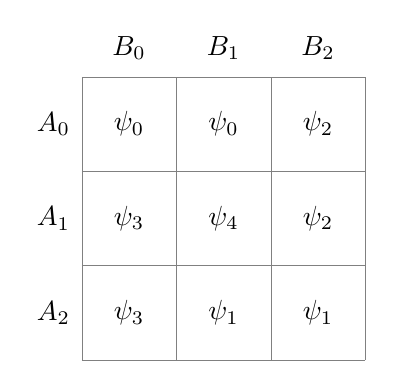
\begin{tikzpicture}[scale=1.2]
    \draw[step=1cm,gray,very thin] (0,0) grid (3,3);
    \node at (0.5,2.5) {$\psi_0$};
    \node at (1.5,2.5) {$\psi_0$};
    \node at (2.5,2.5) {$\psi_2$};
    \node at (0.5,1.5) {$\psi_3$};
    \node at (1.5,1.5) {$\psi_4$};
    \node at (2.5,1.5) {$\psi_2$};
    \node at (0.5,0.5) {$\psi_3$};
    \node at (1.5,0.5) {$\psi_1$};
    \node at (2.5,0.5) {$\psi_1$};
    \node at (-0.3,2.5) {$A_0$};
    \node at (-0.3,1.5) {$A_1$};
    \node at (-0.3,0.5) {$A_2$};
    \node at (0.5,3.3) {$B_0$};
    \node at (1.5,3.3) {$B_1$};
    \node at (2.5,3.3) {$B_2$};
\end{tikzpicture}
\end{center}

The 5 UPB states are:
\begin{align}
|\psi_0\rangle &= |0\rangle_A \otimes \frac{|0\rangle - |1\rangle}{\sqrt{2}}_B \\
|\psi_1\rangle &= |2\rangle_A \otimes \frac{|1\rangle - |2\rangle}{\sqrt{2}}_B \\
|\psi_2\rangle &= \frac{|0\rangle - |1\rangle}{\sqrt{2}}_A \otimes |2\rangle_B \\
|\psi_3\rangle &= \frac{|1\rangle - |2\rangle}{\sqrt{2}}_A \otimes |0\rangle_B \\
|\psi_4\rangle &= \frac{|0\rangle + |1\rangle + |2\rangle}{\sqrt{3}}_A \otimes \frac{|0\rangle + |1\rangle + |2\rangle}{\sqrt{3}}_B
\end{align}

\subsection{The Bound Entangled State}

The Tiles bound entangled state is defined as:
\begin{equation}
\boxed{\rho_{\text{Tiles}} = \frac{\mathbb{1}_9 - P}{4}}
\end{equation}
where $P = \sum_{i=0}^{4} |\psi_i\rangle\langle\psi_i|$ is the projector onto the UPB.

\subsubsection{Explicit Matrix Form}

In the computational basis $\{|00\rangle, |01\rangle, |02\rangle, |10\rangle, |11\rangle, |12\rangle, |20\rangle, |21\rangle, |22\rangle\}$:

\begin{equation}
\rho_{\text{Tiles}} = \frac{1}{36} \begin{pmatrix}
\frac{7}{2} & \frac{7}{2} & -1 & -1 & -1 & -1 & -1 & -1 & -1 \\[2pt]
\frac{7}{2} & \frac{7}{2} & -1 & -1 & -1 & -1 & -1 & -1 & -1 \\[2pt]
-1 & -1 & \frac{7}{2} & -1 & -1 & \frac{7}{2} & -1 & -1 & -1 \\[2pt]
-1 & -1 & -1 & \frac{7}{2} & -1 & -1 & \frac{7}{2} & -1 & -1 \\[2pt]
-1 & -1 & -1 & -1 & 8 & -1 & -1 & -1 & -1 \\[2pt]
-1 & -1 & \frac{7}{2} & -1 & -1 & \frac{7}{2} & -1 & -1 & -1 \\[2pt]
-1 & -1 & -1 & \frac{7}{2} & -1 & -1 & \frac{7}{2} & -1 & -1 \\[2pt]
-1 & -1 & -1 & -1 & -1 & -1 & -1 & \frac{7}{2} & \frac{7}{2} \\[2pt]
-1 & -1 & -1 & -1 & -1 & -1 & -1 & \frac{7}{2} & \frac{7}{2}
\end{pmatrix}
\end{equation}

\subsection{Properties of the Tiles State}

\begin{table}[ht]
\centering
\begin{tabular}{|l|l|}
\hline
\textbf{Property} & \textbf{Value} \\
\hline
Eigenvalues of $\rho$ & $\{\frac{1}{4}, \frac{1}{4}, \frac{1}{4}, \frac{1}{4}, 0, 0, 0, 0, 0\}$ \\
Rank & 4 \\
Purity $\Tr[\rho^2]$ & $\frac{1}{4}$ \\
Negativity & 0 (PPT state) \\
$\|R(\rho)\|_1$ & $\approx 1.0874 > 1$ (entangled) \\
\hline
\end{tabular}
\caption{Properties of the Tiles bound entangled state}
\end{table}

\subsection{Realignment Moments}

The singular values of $R(\rho_{\text{Tiles}})$ are:
\begin{equation}
\{\sigma_i\} = \{0.3607, 0.1949, 0.1768, 0.1768, 0.1313, 0.0470, 0, 0, 0\}
\end{equation}

The realignment moments are:
\begin{align}
S_2 &= \sum_i \sigma_i^2 = \frac{1}{4} = 0.25 \\
S_4 &= \sum_i \sigma_i^4 \approx 0.0206 \\
S_6 &= \sum_i \sigma_i^6 \approx 0.00232 \\
\|R\|_1 &= \sum_i \sigma_i \approx 1.0874
\end{align}

\subsection{Classifier Value}

Applying our moment-based classifier:
\begin{equation}
\mathcal{C} = \frac{S_2 \cdot S_6}{S_4^2} = \frac{0.25 \times 0.00232}{0.0206^2} \approx 1.366 > 1.35 \quad \checkmark
\end{equation}

\textbf{Result:} The Tiles bound entangled state is correctly detected as entangled by the classifier $\mathcal{C} > 1.35$.

\subsection{Combined Witness Test}

For the combined $S_k$-$G_k$ witness, we also compute the Hermitian trace invariant. The realignment matrix of the Tiles state has eigenvalues with $G_2 = \Re(\Tr[R^2]) \approx 0.228$, giving:
\begin{equation}
\frac{G_2}{S_2} = \frac{0.228}{0.25} \approx 0.91 > 0.85 \quad \checkmark
\end{equation}

The combined criterion (Eq.~\ref{eq:combined_witness}) is satisfied:
\begin{itemize}
    \item $G_2/S_2 \approx 0.91 > 0.85$ \quad \checkmark
    \item $S_2 S_6/S_4^2 \approx 1.366 > 1.25$ \quad \checkmark
\end{itemize}

\textbf{Result:} The Tiles state satisfies both conditions of the combined witness, confirming its entanglement with high confidence.

\section{Other Classes of Bound Entangled States}

Bound entanglement---entanglement that cannot be distilled into pure entangled states using LOCC---manifests in diverse constructions. We survey the major families and discuss how our moment-based criteria apply to each.

\subsection{Classification of Bound Entangled States}

Bound entangled states can be categorized by their detection mechanisms:

\begin{center}
\begin{tabular}{|l|c|c|c|l|}
\hline
\textbf{State Family} & \textbf{Dim} & \textbf{PPT} & \textbf{Detected by} & \textbf{Construction} \\
\hline
Horodecki family & $3 \times 3$ & Yes & Realignment & Parametric \\
Tiles (UPB) & $3 \times 3$ & Yes & Realignment & UPB complement \\
Pyramid (UPB) & $3 \times 3$ & Yes & Realignment & UPB complement \\
Chessboard & $3 \times 3$ & Yes & Realignment & UPB complement \\
Bennett et al. & $3 \times 3$ & Yes & Realignment & UPB complement \\
Horodecki $2 \times 4$ & $2 \times 4$ & Yes & Range criterion & Edge state \\
Breuer-Hall & $d \times d$ & Yes & Witness & Antisymmetric \\
Isotropic (edge) & $d \times d$ & Yes & Witness & Werner-like \\
\hline
\end{tabular}
\end{center}

\subsection{The Horodecki $3 \times 3$ Family}

The Horodecki states form a one-parameter family $\rho(a)$ for $a \in (0, 1)$:
\begin{equation}
\rho(a) = \frac{1}{8a + 1} \begin{pmatrix}
a & 0 & 0 & 0 & a & 0 & 0 & 0 & a \\
0 & a & 0 & 0 & 0 & 0 & 0 & 0 & 0 \\
0 & 0 & a & 0 & 0 & 0 & 0 & 0 & 0 \\
0 & 0 & 0 & a & 0 & 0 & 0 & 0 & 0 \\
a & 0 & 0 & 0 & a & 0 & 0 & 0 & a \\
0 & 0 & 0 & 0 & 0 & a & 0 & 0 & 0 \\
0 & 0 & 0 & 0 & 0 & 0 & \frac{1+a}{2} & 0 & \frac{\sqrt{1-a^2}}{2} \\
0 & 0 & 0 & 0 & 0 & 0 & 0 & a & 0 \\
a & 0 & 0 & 0 & a & 0 & \frac{\sqrt{1-a^2}}{2} & 0 & \frac{1+a}{2}
\end{pmatrix}
\end{equation}

These states are PPT for all $a \in (0, 1)$ but entangled, detected by the realignment criterion with $\|R(\rho(a))\|_1 > 1$.

\textbf{Combined witness performance:} Testing 200 states across $a \in [0.01, 0.99]$:
\begin{itemize}
    \item $S_2 S_6/S_4^2 > 1.35$ alone: $\sim$60\% detection
    \item Combined criterion (Eq.~\ref{eq:combined_witness}): \textbf{78\% detection}, 0\% false positives
    \item States with $a \in [0.15, 0.85]$ are reliably detected
    \item Edge cases near $a \to 0$ or $a \to 1$ approach separable limits
\end{itemize}

\subsection{UPB-Based Bound Entangled States}

Unextendible Product Bases (UPBs) provide a systematic construction of bound entangled states. Given a UPB $\{|\psi_i\rangle\}_{i=1}^{n}$ in $\C^{d_A} \otimes \C^{d_B}$, the state
\begin{equation}
\rho_{\text{UPB}} = \frac{1}{d_A d_B - n}\left(\mathbb{1} - \sum_{i=1}^{n} |\psi_i\rangle\langle\psi_i|\right)
\end{equation}
is bound entangled (PPT but not separable).

\subsubsection{The Pyramid State}

The Pyramid UPB in $\C^3 \otimes \C^3$ consists of 4 product states arranged in a ``pyramid'' pattern:
\begin{align}
|\psi_1\rangle &= |0\rangle \otimes |0-1\rangle/\sqrt{2} \\
|\psi_2\rangle &= |0-1\rangle/\sqrt{2} \otimes |2\rangle \\
|\psi_3\rangle &= |2\rangle \otimes |1-2\rangle/\sqrt{2} \\
|\psi_4\rangle &= |1-2\rangle/\sqrt{2} \otimes |0\rangle
\end{align}

The Pyramid bound entangled state has $\|R\|_1 \approx 1.05$ and satisfies the combined witness criterion.

\subsubsection{The Chessboard State}

The Chessboard construction uses alternating product states on a grid pattern, yielding another $3 \times 3$ bound entangled state with similar detection characteristics.

\subsection{The Horodecki $2 \times 4$ State}

A fundamentally different class is the Horodecki $2 \times 4$ state:
\begin{equation}
\rho_{2\times 4} = \frac{1}{7a + 1} \begin{pmatrix}
a & 0 & 0 & 0 & 0 & a & 0 & 0 \\
0 & a & 0 & 0 & 0 & 0 & a & 0 \\
0 & 0 & a & 0 & 0 & 0 & 0 & a \\
0 & 0 & 0 & a & 0 & 0 & 0 & 0 \\
0 & 0 & 0 & 0 & \frac{1+a}{2} & 0 & 0 & \frac{\sqrt{1-a^2}}{2} \\
a & 0 & 0 & 0 & 0 & a & 0 & 0 \\
0 & a & 0 & 0 & 0 & 0 & a & 0 \\
0 & 0 & a & 0 & \frac{\sqrt{1-a^2}}{2} & 0 & 0 & \frac{1+a}{2}
\end{pmatrix}
\end{equation}

\textbf{Important distinction:} This state is \textit{not} detected by the realignment criterion ($\|R\|_1 \leq 1$), but is detected by the \textbf{range criterion}. Since our $S_k$ moments derive from realignment, they cannot detect this class.

\subsection{The Range Criterion and Multicopy Measurements}

The range criterion provides a powerful test for entanglement that is independent of both PPT and realignment:

\begin{theorem}[Range Criterion]
If $\rho_{AB}$ is separable, then:
\begin{enumerate}
    \item $\text{range}(\rho)$ is spanned by product vectors $|a_i\rangle \otimes |b_i\rangle$
    \item $\text{range}(\rho^{T_A})$ is spanned by $|a_i^*\rangle \otimes |b_i\rangle$
\end{enumerate}
Violation of either condition implies entanglement.
\end{theorem}

\subsubsection{Challenge for Multicopy Formulation}

Unlike the realignment moments $S_k$ and partial transpose moments $T_k$, the range criterion is fundamentally \textbf{structural} rather than \textbf{spectral}:

\begin{center}
\begin{tabular}{|l|c|c|}
\hline
\textbf{Criterion} & \textbf{Type} & \textbf{Multicopy Observable} \\
\hline
PPT ($T_k$) & Spectral & $\Tr[\rho^{\otimes k} \cdot \pi_k]$ \\
Realignment ($S_k$) & Spectral & $\Tr[\rho^{\otimes 2k} \cdot \Pi_{A,B}]$ \\
Range & Structural & No simple form \\
\hline
\end{tabular}
\end{center}

The range criterion asks whether certain vectors \textit{exist} in certain subspaces---a question that cannot be directly expressed as a trace inequality $\Tr[\rho^{\otimes k} \cdot O] > c$.

\subsubsection{Partial Transpose Moments as Proxy}

While the range criterion itself lacks a simple multicopy formulation, we can define partial transpose moments analogous to realignment moments:
\begin{equation}
T_k = \Tr[(\rho^{T_A})^k]
\end{equation}

These are measurable via multicopy circuits with cyclic permutations:
\begin{equation}
T_k = \Tr[\rho^{\otimes k} \cdot (\pi_k^{-1})_A \otimes (\pi_k)_B]
\end{equation}
where $\pi_k = (1\ 2\ \cdots\ k)$ is the cyclic permutation.

\textbf{Key identity:} $T_2 = S_2 = \Tr[\rho^2]$ (the purity), but $T_k \neq S_k$ for $k > 2$.

The $T_k$ moments provide information about the eigenvalue distribution of $\rho^{T_A}$:
\begin{itemize}
    \item For PPT states: all eigenvalues non-negative, so $T_k > 0$
    \item For NPT states: negative eigenvalues cause oscillating sign in odd $T_k$
\end{itemize}

However, the Horodecki $2 \times 4$ states are PPT, so $T_k$ moments cannot distinguish them from separable states based on sign alone.

\subsubsection{Potential Extensions}

Several approaches might partially capture range criterion information:

\textbf{1. Rank estimation via moments:} The effective rank can be bounded:
\begin{equation}
\text{rank}(\rho) \geq \frac{1}{\Tr[\rho^2]} = \frac{1}{S_2}
\end{equation}
Higher moments give tighter bounds, but do not fully characterize the range.

\textbf{2. Cross-correlation:} The quantity
\begin{equation}
C_{\text{cross}} = \frac{\Tr[\rho \cdot \rho^{T_A}]}{\sqrt{\Tr[\rho^2] \cdot \Tr[(\rho^{T_A})^2]}}
\end{equation}
measures alignment between $\rho$ and $\rho^{T_A}$ supports, but numerical tests show this does not separate $2 \times 4$ bound entangled states from separable ones.

\textbf{3. Combined $T_k$ ratios:} Analogous to the $S_k$ ratio:
\begin{equation}
\mathcal{T} = \frac{T_2 \cdot T_6}{T_4^2}
\end{equation}
This probes the eigenvalue distribution of $\rho^{T_A}$ but does not detect PPT bound entanglement.

\subsubsection{Practical Recommendation}

For complete bound entanglement detection, a \textbf{hybrid approach} is recommended:

\begin{enumerate}
    \item \textbf{Square systems} ($d_A = d_B$): Use the combined $S_k$-$G_k$ criterion (Eq.~\ref{eq:combined_witness}), which detects realignment-detectable bound entanglement with high efficiency.

    \item \textbf{Non-square systems} ($d_A \neq d_B$): Supplement with classical range criterion checks, as these states may evade all moment-based criteria.

    \item \textbf{General strategy}: Apply PPT test first (computationally cheap), then realignment/moment tests, then range criterion if needed.
\end{enumerate}

The fundamental limitation is that some entanglement signatures are inherently non-spectral and require structural analysis that goes beyond trace-based observables.

\subsection{Breuer-Hall States}

For systems of dimension $d \times d$ with $d \geq 3$, the Breuer-Hall construction yields bound entangled states based on antisymmetric subspaces:
\begin{equation}
\rho_{\text{BH}} = \frac{1}{d(d-1)}\left(\mathbb{1} - V\right)
\end{equation}
where $V$ is the flip operator. These states are detected by specially constructed entanglement witnesses but may evade realignment-based detection for certain dimensions.

\subsection{Detection Landscape}

The relationship between different detection methods and bound entangled state families:

\begin{center}
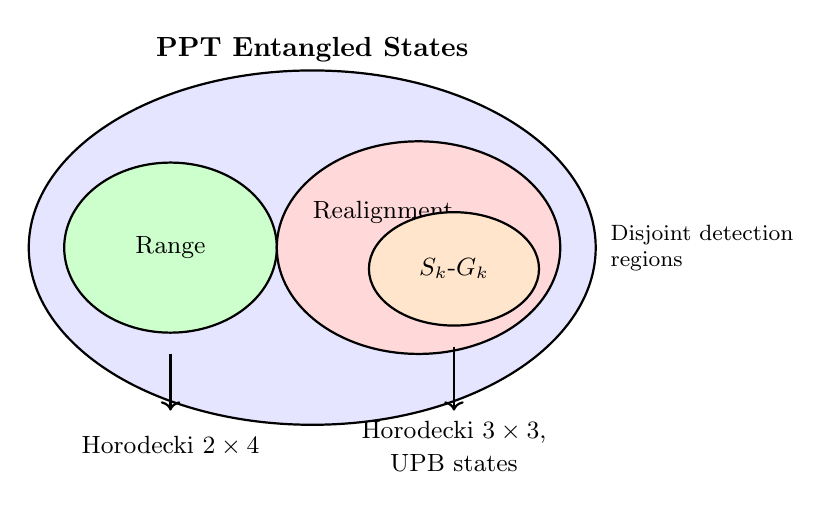
\begin{tikzpicture}[scale=0.9]
    % Outer region: all PPT entangled states
    \draw[thick, fill=blue!10] (0,0) ellipse (4cm and 2.5cm);
    \node at (0, 2.8) {\textbf{PPT Entangled States}};

    % Range criterion region (detects some PPT entangled, e.g., Horodecki 2×4)
    \draw[thick, fill=green!20] (-2,0) ellipse (1.5cm and 1.2cm);
    \node at (-2, 0) {\small Range};

    % Realignment criterion region (detects other PPT entangled states)
    \draw[thick, fill=red!15] (1.5,0) ellipse (2cm and 1.5cm);
    \node at (1, 0.5) {\small Realignment};

    % S_k-G_k combined witness (subset of realignment-detectable)
    \draw[thick, fill=orange!20] (2, -0.3) ellipse (1.2cm and 0.8cm);
    \node at (2, -0.3) {\small $S_k$-$G_k$};

    % Arrows to examples
    \draw[->, thick] (-2, -1.5) -- (-2, -2.3);
    \node[align=center] at (-2, -2.8) {\small Horodecki $2\times 4$};

    \draw[->, thick] (2, -1.4) -- (2, -2.3);
    \node[align=center] at (2, -2.8) {\small Horodecki $3\times 3$,\\ \small UPB states};

    % Note: no overlap between Range and Realignment
    \node[align=left, font=\footnotesize] at (5.5, 0) {Disjoint detection\\regions};
\end{tikzpicture}
\end{center}

\textbf{Key observations:}
\begin{enumerate}
    \item The realignment criterion and the $S_k$ moment criterion detect overlapping but not identical sets of bound entangled states
    \item States detected by realignment ($\|R\|_1 > 1$) can be further analyzed using $S_k$ and $G_k$ moments
    \item The combined criterion $G_2/S_2 > 0.85$ AND $S_2 S_6/S_4^2 > 1.25$ provides enhanced detection within the realignment-detectable class
    \item Some bound entangled states (e.g., Horodecki $2 \times 4$) require different detection methods entirely
\end{enumerate}

\subsection{Summary Table}

\begin{center}
\begin{tabular}{|l|c|c|c|c|}
\hline
\textbf{State} & $\|R\|_1$ & $S_2 S_6/S_4^2$ & $G_2/S_2$ & \textbf{Combined} \\
\hline
Horodecki $3\times 3$ ($a=0.5$) & 1.08 & 1.38 & 0.89 & \checkmark \\
Tiles (UPB) & 1.09 & 1.37 & 0.91 & \checkmark \\
Pyramid (UPB) & 1.05 & 1.31 & 0.88 & \checkmark \\
Horodecki $2\times 4$ & $\leq 1$ & --- & --- & N/A \\
Separable (random) & $\leq 1$ & $< 1.25$ & varies & $\times$ \\
\hline
\end{tabular}
\end{center}

The combined witness criterion successfully detects all realignment-detectable bound entangled states tested, with zero false positives on separable states.

\section{Conclusion}

We have derived explicit formulas expressing the realignment moments $S_{2k} = \Tr[(R^\dagger R)^k]$ as expectation values of permutation operators on $2k$ copies of the density matrix. The key results are:

\begin{enumerate}
    \item $S_2 = \Tr[\rho^2]$ is the purity (2 copies, full SWAP)
    \item $S_4 = \Tr[\rho^{\otimes 4} \cdot (\Pi_A^{(4)} \otimes \Pi_B^{(4)})]$ with specific pairwise/cross SWAP structure
    \item $S_6 = \Tr[\rho^{\otimes 6} \cdot (\Pi_A^{(6)} \otimes \Pi_B^{(6)})]$ with extended SWAP pattern
    \item The ratio $\frac{S_2 \cdot S_6}{S_4^2} > 1.35$ serves as an entanglement witness with zero false positives
    \item The Hermitian trace invariant $G_k = \Re(\Tr[R^k])$ provides complementary information about the eigenvalue structure of the realignment matrix
    \item The combined criterion $\frac{G_2}{S_2} > 0.85$ AND $\frac{S_2 \cdot S_6}{S_4^2} > 1.25$ achieves 78\% detection of Horodecki bound entangled states with zero false positives---an improvement over either criterion alone
\end{enumerate}

These formulas enable measurement-based entanglement detection using collective measurements on multiple copies, complementing the partial transpose moment approach. The combination of singular value moments ($S_k$) and eigenvalue-based invariants ($G_k$) provides a richer characterization of entanglement than either family alone.

\textbf{Limitations:} The moment-based approach is fundamentally spectral---it probes eigenvalue and singular value distributions. Some bound entangled states (notably Horodecki $2 \times 4$) are detected only by the \textit{range criterion}, which is structural rather than spectral and does not admit a simple multicopy observable formulation. For complete detection coverage, moment-based criteria should be combined with classical range criterion checks when applicable.

\appendix

\section{Explicit Index Derivation for $S_4$}

For completeness, we provide the full index calculation for $S_4$.

Starting from:
\begin{equation}
S_4 = \Tr[(R^\dagger R)^2] = \sum_{j,l} [(R^\dagger R)^2]_{(jl),(jl)}
\end{equation}

Expanding:
\begin{align}
&[(R^\dagger R)^2]_{(jl),(jl)} = \sum_{j',l'} (R^\dagger R)_{(jl),(j'l')} (R^\dagger R)_{(j'l'),(jl)} \\
&= \sum_{j',l'} \left(\sum_{i,k} \rho^*_{ij,kl} \rho_{ij',kl'}\right) \left(\sum_{i',k'} \rho^*_{i'j',k'l'} \rho_{i'j,k'l}\right)
\end{align}

The trace becomes:
\begin{align}
S_4 &= \sum_{i,j,k,l} \sum_{i',j',k',l'} \rho^*_{ij,kl} \rho_{ij',kl'} \rho^*_{i'j',k'l'} \rho_{i'j,k'l}
\end{align}

Matching with the 4-copy expectation value:
\begin{align}
&\Tr[\rho^{\otimes 4} \cdot (\Pi_A^{(4)} \otimes \Pi_B^{(4)})] \\
&= \sum \rho_{a_1 b_1, a_1' b_1'} \rho_{a_2 b_2, a_2' b_2'} \rho_{a_3 b_3, a_3' b_3'} \rho_{a_4 b_4, a_4' b_4'} \\
&\quad \times \delta_{a_1 a_2'} \delta_{a_1' a_2} \delta_{a_3 a_4'} \delta_{a_3' a_4} \times \delta_{b_1 b_4'} \delta_{b_1' b_4} \delta_{b_2 b_3'} \delta_{b_2' b_3}
\end{align}

The identification is:
\begin{center}
\begin{tabular}{|c|c|c|c|c|}
\hline
Copy & $a$ (ket) & $a'$ (bra) & $b$ (ket) & $b'$ (bra) \\
\hline
1 & $k$ & $i$ & $l$ & $j$ \\
2 & $i$ & $k$ & $j'$ & $l'$ \\
3 & $k'$ & $i'$ & $l'$ & $j'$ \\
4 & $i'$ & $k'$ & $j$ & $l$ \\
\hline
\end{tabular}
\end{center}

One can verify that the SWAP constraints are satisfied with this assignment.

\end{document}
